L'ultima tipologia di rivelatore che trattiamo sono i rivelatori a semiconduttore, detti anche rivelatori a stato solido. Questi rivelatori si basano sull'utilizzo di materiali semiconduttori, i quali sono dei materiali cristallini cioè costituiti da una struttura ordinata di atomi in un reticolo, in particolare i primi che sono stati inventati si basano sull'utilizzo di silicio o germanio.

Sono anche detti rivelatori a stato solido, perché hanno una densità che è circa mille volte maggiore rispetto a quella dei gas. Ciò costituisce una notevole differenza rispetto ai rivelatori a gas, i quali si basano sull'utilizzo di un gas a densità molto basse, mentre qui abbiamo un materiale solido e questo comporta delle differenze nelle caratteristiche che andremo ad approfondire.

\section{Semiconduttori puri}
I primi rivelatori che ormai hanno una loro storia: i primi prototipi sono stati sviluppati negli anni '60, da allora ci sono stati enormi sviluppi e oggi abbiamo rivelatori al silicio particolarmente performanti pensati per diversi tipi di applicazione, per cui in questo capitolo introdurremo il concetto di base di rivelazione basata sul semiconduttore, cioè come è stato inventato il rivelatore dal semiconduttore, per poi vedere alla fine alcune applicazioni e alcuni esempi di come i rivelatori al semiconduttore sono stati sviluppati e migliorati nel corso degli anni.

\subsection{Vantaggi e svantaggi}

I rivelatori a semiconduttore hanno diversi vantaggi:
\begin{itemize}[leftmargin=0.5cm]
   \item Hanno un'ottima risoluzione energetica.\\
   Durante il primo ciclo di esperienze è stato possibile misurare la risoluzione in energia\footnote{Ricordiamo che la risoluzione in energia esprime la capacità di un rivelatore di distinguere due valori in energia molto vicini tra di loro, per cui se la risoluzione non è buona quello che succede è che si rischia di non riuscire a distinguere due valori in energia molto vicini tra di loro.} con un rivelatore a scintillazione. In tale esperienza si hanno degli spettri acquisiti utilizzando le sorgenti $\gamma$, e andando a guardare la larghezza del picco fotoelettrico è possibile valutare la risoluzione in energia. Svolgendo tale operazione, ci si rende conto che un sistema basato sull'utilizzo di uno scintillatore e di un fotomoltiplicatore porta ad avere risoluzioni in energia che non sono particolarmente spinte, dell'ordine del 5-10\%. I rivelatori a semi-conduttore invece presentano delle buone risoluzioni energetiche;
   \item Hanno elevato stopping power.\\
   Infatti il fatto di avere a disposizione un materiale solido fa sì che la radiazione che penetra all'interno del rivelatore venga più facilmente arrestata, quindi perda più facilmente energia. Pensiamo ad esempio alla perdita di energia di un elettrone che deve entrare in un rivelatore a gas oppure in un rivelatore a silicio: nel rivelatore a silicio percorre veramente pochi millimetri, in un rivelatore a gas potrebbe percorre diversi centimetri. Quindi questo fa sì che affinché ad esempio il rivelatore venga utilizzato per misurare tutta l'energia di una particella sono sufficienti spessori e dimensioni compatte. Ad esempio in laboratorio utilizziamo questi rivelatori per misurare particelle $\alpha$ da 5 meV, le quali vengono arrestate in poche decine di micron di silicio, quindi è sufficiente un rivelatore spesso $50 \; \rm \mu m$ come quello che utilizziamo in laboratorio per essere sicuri che le particelle $\alpha$ vengano arrestate all'interno del rivelatore, quindi ne misuriamo tutta l'energia;
   \item In generale questi rivelatori, che sono sostanzialmente delle raggiunzioni P-N polarizzate inversamente, richiedono delle basse tensioni di alimentazione, il che costituisce un vantaggio da un punto di vista pratico.\\
   Se facciamo un confronto con i fotomoltiplicatori che richiedono centinaia di Volt, o anche con il contatore Geiger, nel quale si adoperano tensioni dell'ordine di $300-400$ Volt, per il rivelatore al silicio sono sufficienti tensioni molto più piccole, dell'ordine di decine di Volt per la polarizzazione.
   \item Hanno una risposta abbastanza veloce, cosa che invece non avevamo per i rivelatori a gas, i quali sono dei rivelatori piuttosto solenti proprio per i meccanismi e i fenomeni che avvengono al loro interno. Ciò è utile soprattutto per le misure di timing.
\end{itemize}

Tuttavia ci sono anche degli svantaggi:
\begin{itemize}[leftmargin=0.5cm]
   \item Il principale svantaggio è il fatto che questi rivelatori sono parecchio sensibili alla temperatura, quindi le condizioni di lavoro possono cambiare a seconda della temperatura in cui si sta operando. A volte alcuni di questi richiedono addirittura un sistema di raffreddamento perché altrimenti il rumore sarebbe eccessivamente elevato. \E il caso dei rivelatori al germanio, i quali necessitano di un raffreddamento;
   \item Il danneggiamento da radiazione. Infatti, essendo il semiconduttore composto da un reticolo, cioè da una struttura ordinata, quando viene sottoposto a un'elevata dose di radiazione questa dose può produrre dei danni al reticolo, quindi modificare in qualche modo la struttura ordinata del reticolo e causare delle conseguenze sul funzionamento del rivelatore. Ciò non costituisce un problema per le esperienze che svolgiamo in laboratorio dal momento che noi utilizziamo una sorgente $\alpha$ che ha un'attività abbastanza bassa. Questi problemi si presentano laddove questi rivelatori devono essere adoperati in presenza di alte radiazioni, come nel caso di esperimenti sotto fascio dunque in un acceleratore, oppure esperimenti nello spazio dove la radiazione cosmica diventa importante perché non si è più schermati dal filtro dovuto all'atmosfera terrestre;
   \item Dimensioni compatte. Tale aspetto può costituire uno svantaggio, in quanto dover rivestire una superficie molte estesa con un rivelatore a semiconduttore è estremamente costoso e anche impegnativo dal punto di vista di elettronica e del consumo, per cui quando si deve realizzare un rivelatore a semiconduttore di dimensioni estese, nascono altre problematiche e può essere non facile affrontarle.
\end{itemize}

\subsection{Banda di valenza e banda di conduzione}
Richiamiamo velocemente le proprietà dei semiconduttori.

I materiali solidi si distinguono in tre categorie diverse a seconda dello struttura a bande dei livelli di energia:
\begin{figure}[H]
   \centering
   \includegraphics[width=0.9\textwidth]{immagini/bande_valenza_e_conduzione.png}
\end{figure}
In generale se banda di valenze e quella di conduzione sono separati da un gap abbastanza esteso in cui non possono essere presenti dei livelli energetici, una gap di energia proibita, abbiamo un materiale isolante, mentre il gap è inesistente abbiamo un materiale conduttore. Una situazione intermedia è quella dei materiali semiconduttori, dove questa gap è presente  però non ha una dimensione molto grande, dell'ordine di alcuni electron volt quindi esiste ma è abbastanza piccola.

Vediamo che succede se applichiamo un campo elettrico a queste tre tipologie di materiale:
\begin{itemize}[leftmargin=0.5cm]
   \item In un isolante non comporta il passaggio di corrente, perché tutti gli elettroni si trovano nella banda di valenza e quindi non abbiano conduzione;
   \item In un conduttore si osserva il passaggio di una corrente;
   \item In un semiconduttore si osserva una piccolissima corrente legata al fatto che alcuni elettroni, che definiamo elettroni termici i quali hanno acquisito un'energia per efetti termici sufficiente a superare il gap energetico, possono condurre. \E chiaro che è un effetto puramente statistico, dovuto all'agitazione termica, quindi si genera una corrente abbastanza debole.
\end{itemize}
Nei semiconduttori abbiamo un'altra caratteristica fondamentale, cioè il fatto che i portatori di carica, cioè le cariche che generano una corrente possono essere di due tipologie, \textit{elettroni} e \textit{lacune}.
\begin{figure}[H]
   \centering
   \includegraphics[width=0.9\textwidth]{immagini/elettroni_e_lacune_semiconduttori.png}
\end{figure}
Le lacune sono delle vacanze di elettroni e anch'esse concorrono al valore della corrente in un semiconduttore, quindi ogni volta che noi andremo a parlare di questi effetti di corrente, faremo riferimento sia elettroni che lacune.

\subsection{Creazione di coppie}

Normalmente, in un semiconduttore esistono due fenomeni che sono in competizione l'uno con l'altro:

\begin{enumerate}[leftmargin=0.6cm]
   \item Creazione di coppie elettrone-lacuna che abbiamo già accennato, cioè per effetti termici effettivamente un elettrone potrebbe passare dalla banda di valenza alla banda di conduzione e quindi si viene a creare una coppia elettrone-lacuna;
   \item Ricombinazione, cioè un elettrone potrebbe ricombinarsi con una lacuna, purché i valori di energia e di impulso lo consentono.
\end{enumerate}

Analizziamo il primo fenomeno. \E chiaro che in generale, in un semiconduttore puro, detto anche in trinceco\footnote{Da non confondere con il semiconduttore intrinseco visto negli APD.}, il numero di elettroni che si trova nella banda di conduzione è esattamente uguale al numero delle lacune in banda di valenza, perché ogni volta che un elettrone viene promosso salta dalla banda di valenza alla banda di conduzione e crea la sua lacuna corrispondente. Sia gli elettroni che le lacune contribuiscono alla conducibilità elettrica del semiconduttore. 

Cerchiamo allora di capire quanto vale la concentrazione di elettroni e di lacune. Dal momento che stiamo considerando un semiconduttore puro, il numero di elettroni corrisponde al numero di lacunhe, dunque indichiamo la concentrazione in generale con $n_i$, che sarà data da
\begin{equation*}
   n_i
   =\sqrt{N_C N_V} \exp{ -\frac{E_g}{2k_B T} }
   =AT^{\frac{3}{2}} \exp{ -\frac{E_g}{2k_B T} }
\end{equation*}
dove
\begin{itemize}[leftmargin=0.5cm]
   \item $N_C$ e $N_v$ sono rispettivamente il numero di possibili stati nella banda di conduzione e in quella di valenza;
   \item $E_g$ è l'energia della gap proibita;
   \item $T$ è la temperatura;
   \item $k_B$ è la costante di Boltzmann
   \item $A$ è una costante indipendente dalla temperatura
\end{itemize}

Le dipendenze dall'energia della gap e dalla temperatura nell'esponenziale decrescente sono abbastanza intuitive: per quanto riguarda $E_g$, se la gap è piccola per un elettrone sarà più facile lasciare la banda di valenza e andare verso la banda di conduzione, viceversa più è elevata la temperatura più sarà probabile che un elettrone possa passare alla banda di conduzione per effetto termico, ecco perché lo si trova al denominatore. Utilizzando la statistica di Fermi-Dirac, è possibile inoltre valutare il numero di stati nella banda di conduzione e dalla banda di valenza. Si trova che il loro prodotto è pari a $N_C N_V=AT^3$. In definitiva, la concentrazione di elettroni e lacune libere dovuto soltanto all'effetto termico dipende dalle caratteristiche del semiconduttore (in particolare da $E_g$) e dalla temperatura $T$. 

Vediamo quanti elettroni e lacune abbiamo a temperatura ambiente per due semiconduttori, silicio e germanio, i quali si differiscono per le dimensioni della gap. Supposto di avere una temperatura di 300 K, troviamo una concentrazione di $2.5 \cdot 10^{13}/\rm cm^3$ per il germanio e $1.5 \cdot 10^{10}/\rm cm^3$ per il silicio. Se consideriamo che in media abbiamo $10^{22} \text{ atomi/cm}^3$, tali valori corrispondono rispettivamente a dire che soltanto un elettrone su $10^9$ atomi per il germanio un elettrone su $10^{12}$ atomi per il silcio si trova nella banda di conduzione, quindi effettivamente non sono tantissimi. Ciò ha una corrispondenza con quanto affermato prima, ossia che se applichiamo un campo elettrico a un materiale semiconduttore si genera una corrente molto piccola, ed effettivamente è così perché troviamo poche coppie elettrone-lacune dovute ad effetti termici.
\subsection{mobilità}
Sotto l'azione di un campo elettrico $E$, elettroni e lacune cominciano a muoversi, cioè subiscono un moto di deriva. Possiamo valutare le velocità con cui avviene questa deriva: esse sono date da\footnote{Il pedice $h$ sta per "hole", cioè lacuna in inglese.}
\begin{equation*}
   v_e=\mu_e E
   \qq{,}
   v_h=\mu_h E
\end{equation*}
Come possiamo vedere, le velocità di elettroni e lacune sono proporzionali al valore del campo elettrico e alla mobilità, che sono diverse per elettroni e lacune. Queste mobilità non sono costanti, dipendono dal valore del campo elettrico e della temperatura, ad esempio per il silicio a temperature normali troviamo che le mobilità $\mu_e$ e $\mu_h$:
\begin{itemize}[leftmargin=0.5cm]
   \item risultano essere costanti per valori di campo elettrico inferiori a $10^3 \; \rm V/cm$;
   \item hanno una dipende del tipo $E^{-\frac{1}{2}}$ per valori di campo elettrico compresi tra $10^3-10^4 \; \rm V/cm$;
   \item hanno una dipende del tipo $E^{-1}$ per valori di campo maggiori di $10^4 \; \rm V/cm$.
\end{itemize}
Tale andamento ha come conseguenza il fatto che arrivati a un certo punto si giunge a una saturazione della velocità a un valore massimo di $10^7$ cm/s, legato al fatto che l'energia che viene acquisita da questi elettroni e queste lacune viene poi persa per gli urti con il reticolo.

Alla luce di quanto visto, la conduttività di un semiconduttore si può esprimere considerando sia il contributo dovuto agli elettroni che quello dovuto alle lacune:
\begin{equation*}
   \sigma=e n_i (\mu_e + \mu_h)
\end{equation*}
\subsection{Ricombinazione e trapping}

Può avvenire una ricombinazione spontanea, cioè legata al fatto che elettrone e lacune aventi opportuni valori di energia ed impulso possono ricombinarsi e dare luogo all'emissione di un fotone. Tale processo è un meccanismo raro, perché non è sufficiente che elettroni e lacune si trovino vicine per ricombinarsi, ma devono avere anche dei valori opportuni di energia e impulso. A riprova della sua rarità, la vita media di una coppia che è stata creata per effetti termici è dell'ordine di un secondo, dopodiché per qualche motivo c'è una ricombinazione e tale coppia cessa di esistere. Sebbene un secondo possa sembrare un tempo piccolo, se confrontato con i tempi caratteristici dei rivelatori risulta essere un tempo enorme, dunque questa coppia sopravvive parecchio.

Tuttavia quello che si osserva sperimentalmente è che la vita media di una coppia è molto più bassa di un secondo, quindi evidentemente ci sono altri meccanismi oltre alla ricombinazione spontanea che portano alla scomparsa della coppia. Questi meccanismi sono legati alla presenza dei centri di ricombinazione.

\begin{figure}[H]
   \centering
   \includegraphics[width=0.55\textwidth]{immagini/centri_di_ricombinazione.png}
\end{figure}

Infatti, a causa di difetti della struttura cristallina si possono presentare dei livelli nella zona proibita, i quali sono dei livelli che vengono definiti profondi nel senso che sono abbastanza distanziati sia dalla banda di conduzione che dalla banda di valenza (lo possiamo vedere tratteggiati in figura). In questi livelli si può verificare una ricombinazione perché sono livelli che possono attrarre elettroni dalla banda di conduzione e lacune della banda di valenza permettendo quindi una ricombinazione. Ecco perché vengono definiti come centri di ricombinazione.

Tali centri di ricombinazione fanno sì che alla fine la vita media di una coppia sia effettivamente più bassa.

\vspace{0.2cm}Da un punto di vista della rivelazione, visto che il rivelatore a semiconduttore produce per effetto del passaggio di una particella coppie elettrone-lacuna su cui si basa il segnale, ci interessa che tali coppie non si ricombinino prima di riuscire a raccoglierle, dunque non vogliamo che la vita media sia eccessivamente bassa perché se queste coppie si ricombinano troppo rapidamente perdiamo il segnale. In conseguenza a ciò i semiconduttori che adoperiamo nei rivelatori devono essere estremamente puri, cioè devono presentare pochi difetti perché più difetti ci sono più aumentano i centri di ricombinazione.

Alcuni centri di ricombinazione sono anche definiti dei centri trappola. Sono dei livelli dove viene catturata soltanto una tipologia di carica, quindi ad esempio viene catturato un elettrone dalla banda di conduzione e l'elettrone rimane in tale sito per parecchio tempo, da cui il nome livelli trappola.

\vspace{0.2cm}Vediamo ora che tipo di difetti possono essere presenti in un reticolo cristallino come quello di un semiconduttore
\begin{figure}[H]
   \centering
   \includegraphics[width=0.7\textwidth]{immagini/difetti_cristallini.png}
\end{figure}
In questa figura sono rappresentate i principali difetti di un reticolo:
\begin{itemize}[leftmargin=0.5cm]
   \item Potremmo avere una vacanza, cioè l'assenza di un atomo che era previsto nel reticolo;
   \item Potremmo avere un difetto è autointerstiziale, che è l'opposto della vacanza, in quanto si ha un atomo dello stesso tipo del cristallo in più rispetto a quanto previsto dello schema del reticolo;
   \item Potremmo avere un difetto interstiziale, che si differenze dal precedente per il fatto che abbiamo sempre un atomo in più rispetto a quanto previsto però è un atomo di natura diversa;
   \item Potremmo infine avere dei difetti sostituzionali, cioè un atomo del semiconduttore viene sostituito con un atomo di tipologia diversa, però affinché ciò avvenga le dimensioni devono essere abbastanza simili, dunque i raggi dei due automi devono essere similari.
\end{itemize}
Ogni difetto del reticolo comporta una modifica nello schema dei livelli energetici. Scegliendo però in maniera opportuna degli elementi da aggiungere al reticolo cristallino, ossia con opportuni drogaggi, possiamo generare degli ulteriori livelli energetici superficiali, ossia livelli che sono vicini o alla banda di conduzione o alla banda di valenza. Per questo motivo nella pratica si utilizzano semiconduttori drogati.

\section{Semiconduttori drogati}
In un semiconduttore drogato, detto anche semiconduttoro estrinseco, si vanno a sostituire gli atomi del semiconduttore con atomi di elementi diversi. Ad esempio, caso di silicio e germanio, i quali sono entrambi tetravalenti cioè hanno quattro elettroni di valenza, per drogarli è necessario introdurre atomi trivalenti o atomi pentavalenti.

La conseguenza del drogaggio è una variazione nella proporzione tra elettroni e lacune. Infatti in un semiconduttore puro il numero di elettroni coincide con il numero delle lacune generati per effetti termici, mentre drogando il materiale creiamo uno squilibrio.

\subsection{Semiconduttori di tipo n}
In un semiconduttore drogato di tipo n si va a sostituire un atomo del reticolo con un atomo pentavalente, come ad esempio l'arsenico, il fosforo o l'antimonio.
\begin{figure}[H]
   \centering
   \includegraphics[width=0.8\textwidth]{immagini/semiconduttori_drogati_tipo_n.png}
\end{figure}
Questo atomo avrà 5 elettroni di cui 4 vanno a legarsi con i quattro atomi di sitiscio che si tromano attorno, mentre il quinto elettrone rimane in eccesso e può essere un elettrone di conduzione. L'aggiunta di un tale atomo corrisponde a generare nella zona del gap proibito di energie un livello superficiale, che in questo caso è molto vicino alla banda di conduzione, a una distanza di 0,01 eV nel caso del Germania o 0,05 eV nel caso del silicio. Questo elettrone si troverà in questo livello discreto, per cui gli sarà sufficiente una piccolissima energia per essere in grado di passare alla banda di conduzione, quindi sostanzialmente è un elettrone quasi libero.

Con valori di drogaggio tipici si può raggiungere un numero di elettroni di conduzione di $10^{17}\text{ elettroni/cm}^3$, mentre il numero di lacune si riduce a $10^3\text{ lacune/cm}^3$. Ecco perché nei simiconduttori drogati di tipo n i portatori di carica maggioritari sono gli elettroni mentre le lacune rappresentano i portatori di carica minoritari.
\subsection{Semiconduttori di tipo p}
La situazione è diamentralmente opposta in simiconduttore drogato di tipo p. In questo caso si va a sostituire un atomo del reticolo con un atomo trivalente come il gallio, il borro o l'indio e quello che stavolta rimane in eccesso è una lacuna.
\begin{figure}[H]
   \centering
   \includegraphics[width=0.8\textwidth]{immagini/semiconduttori_drogati_tipo_p.png}
\end{figure}

Questa lacuna si troverà in un livello discreto situato nella banda di energia probita, a una distanza molto piccola dalla banda di valenza. In questo caso le lacune rappresentano i portatori di carica maggioritari e gli elettroni quelli minoritari.

Va precisato che anche se introduciamo un'impurezza ossia un atomo di tipo diverso, il materiale rimane comunque neutro. Infatti nel caso in cui ad esempio introduciamo un'impurità di tipo n cioè un donore, sebbene ci sia un elettrone in eccesso ciò non vuol dire che il materiale è carico negativamente, perché abbiamo la carica del nucleo che compensa l'elettrone libero. ne segue che complessivamente abbiamo un materiale neutro. Analoghi ragionamenti valgono nel caso in cui introduciamo un atomo accettore.

\subsection{Concentrazione di elettroni e lacune}
Si può dimostrare che, indipendentemente del tipo di drogaggio, il prodotto della concentrazione di elettroni $n$ per la concentrazione di lacune $p$ è sempre data da
\begin{equation*}
   np=n_i^2
\end{equation*}
dove $n_i$ è la concentrazione nel caso del semiconduttore intrinseco.

Da tale relazione segue che se aumentano gli elettroni per effetto di un drogaggio, la quantità delle lacune che si formano nel semiconduttore non rimane costante ma diminuisce e viceversa nel caso opposto. 

La legge appena enunciata prende il nome di legge dell'azione di massa. Partendo da tale legge, in un semiconduttore di tipo n, dove ci aspettiamo che il numero di atomi accettori $N_A$ sia pari a zero mentre il numero di atomi donori $N_D$ comporti la formazione di un medesimo numero di elettroni\footnote{Gli atomi accettori e donori sono rispettivamente elementi che accettano elettroni e donano elettroni dal/al semiconduttore.}, possiamo esprimere la concentrazione di lacune e la conducibilità del materiale come segue:
\begin{equation*}
   p \approx \frac{n_i^2}{N_D}
   \qq{e}
   \sigma \approx e N_D \mu_e
\end{equation*}
Analogamente, per un simiconduttore drogato di tipo p, dove stavolta abbiamo $N_D=0$ e $N_A$ lacune, abbiamo 
\begin{equation*}
   n \approx \frac{n_i^2}{N_A}
   \qq{e}
   \sigma \approx e N_A \mu_h
\end{equation*}
Vediamo come a differenza di prima, dove la conducibilità veniva espressa come somma di due termini, uno dovuto agli elettroni e uno dovuto alle lacune, nel caso di semiconduttori drogati la conduzione elettrica è affidata ai portatori maggioritari di carica, ossia gli elettroni nel caso dei simiconduttori drogati di tipo N e le lacune nei casi semiconduttori drogati di tipo P. Se allora vogliamo avere una corrente più elevata, quello che dovete fare è drogare maggiormente il materiale, per cui se ad esempio abbiamo un drogaggio di tipo n dobbiamo aumentare la concentrazione degli atomi donori; viceversa nel simiconduttore di tipo p dobbiamo aumentare la concentrazione di atomi acettori.

\subsection[Semiconduttori di tipo \texorpdfstring{$\rm p+$}{p+}, \texorpdfstring{$\rm p-$}{p-}, i (compensati)]
{Semiconduttori di tipo $\boldsymbol{\rm p+}$, $\boldsymbol{\rm p-}$, i (compensati)}
Può essere utile drogare i semiconduttori con elevate concentrazioni, anche dell'ordine di $10^{20}\text{ atomi/cm}^3$ anziché i soliti $10^{13}\text{ atomi/cm}^3$. Per quanto detto prima, questi materiali risultano essere altamente conduttivi. Inoltre essi sono indicati con il simbolo "$+$" proprio per indicare che la concentrazione è elevata e vengono tipicamente adoperati per la realizzazione dei contatti elettrici. Infatti in qualsiasi rivelatore per poter estrarre un segnale elettrico abbiamo bisogno di contatti elettrici, ad esempio nel caso del rivelatore a gas abbiamo anodo e catodo da cui possiamo prelevare un segnale. Qui il materiale semiconduttore non ha dei contatti, dunque bisogna crearli, sebbene ciò non sia facile crearli perché nel momento in cui proviamo a utilizzare un materiale metallico a contatto con un semiconduttore purtroppo introduciamo degli effetti collaterali. Per evitare ciò, quello che si fa è realizzare delle zone ad alto drogaggio proprio là dove vogliamo creare il contatto ohmico con un metallo.

Per quanto riguarda i semiconduttori etichettati con la lettere "i", ingenuamente potremmo pensare che stia per intrinseco, ma in realtà non è esattamente così. Infatti un materiale di tipo i si comporta come un materiale intrinseco cioè un materiale puro, ma in realtà prende il nome di materiale compensato, perché è comunque un semiconduttore che è stato drogato, sia di tipo n che di tipo p, con la stessa concentrazione. L'effetto risultante di tale drogaggio è dunque quello di riportare il semiconduttore alla condizione di intrinseco, ma bisogna sempre ricordare che è stato drogato. Sono materiali che hanno una resistività elevata.

\subsection{Giunzioni n-p}
Il principio di base di un rivelatore a semiconduttore sono le giunzioni p-n o n-p. Se prendiamo due materiali, uno drogato di tipo n e uno drogato di tipo p, e li accostiamo uno vicino all'altro, avvengono dei fenomeni. 
\begin{figure}[H]
   \centering
   \includegraphics[width=0.8\textwidth]{immagini/giunzione_p-n.png}
\end{figure}
Poiché stiamo mettendo a contatto dei materiali che hanno concentrazione di carica diverse l'uno dall'altro (nel materiale di tipo n c'è un'elevata concentrazione di elettroni liberi, mentre nel materiale di tipo p c'è un'elevata concentrazione di lacune), si verifica una diffusione di elettroni verso il materiale di tipo p e di lacune verso il materiale di tipo n, proprio a causa di questa differente concentrazione. Gli elettroni che si diffondono nella zona di tipo p incontrano le lacune e si ricombinano con queste; lo stesso avviene nel materiale di tipo n, dove le lacune che si sono diffuse in esso si ricombinano con gli elettroni. Essendo entrambe le zone n e p inizialmente neutre, nella giunzione la zona n avrà una concentrazione di cariche positive mentre la zona p di cariche negative. Come possiamo infatti vedere dalla figura a), inizialmente in n erano presenti gli elettroni liberi mentre in n le lacune, e una volta realizzata la giunzione gli elettroni sono passati da n a p e si sono ricombinati con le lacune. In conseguenza a ciò, nella regione p sono rimasti degli ioni negativi, fissi nel reticolo. viceversa nella zona di tipo n, le lacune si sono ricombinate con gli elettroni e quindi sono rimasti fissi nel reticolo gli ioni positivi. Ciò comporta la formazione di un campo elettrico e dunque di un potenziale $V_0$, detto potenziale di contatto, che come possiamo vedere nella figura b), dove sull'asse verticale sono riportati i livelli in energia mentre l'asse orizzontale la posizione in corrispondenza con la figura a), ha deformato i livelli energetici. In altri termini, a causa della presenza di queste cariche fisse nel reticolo dei materiali di tipo p e di tipo n, si è creata una differenza di potenziale che impedisce l'ulteriore passaggio e diffusione di cariche libere. Si è allora creata una regione che dal punto di vista della rivelazione è ottimale, perché è una regione in cui non sta circolando carica libera e quindi se per caso dovesse passare una particella, la quale comporta la formazione di nuove cariche, quest'ultime possono essere spazzate via da questo potenziale e raccolte.

Il potenziale di contatto $V_0$ è abbastanza piccolo, circa $1 \; \rm V$. Inoltre la zona che si è venuta a creare prende il nome di zona di svuotamento, perché è una zona dove abbiamo eliminato tutte le cariche libere. Sono quindi presenti delle cariche fisse, che determinano un campo elettrico, ma non sono presenti cariche libere che potrebbero rappresentare rumore per i nostri scopi, in quanto sono cariche che non sono dettate dal passaggio di una radiazione, ma sono cariche che erano presenti nel materiale semiconduttore. Non essendo presenti in questa regione, essa risulta essere una regione utile per la rivelazione.

Cerchiamo allora di valutare l'estensione di tale regione. Per fare ciò consideriamo la concentrazione degli atomi accettori e degli atomi donori\footnote{La dimostrazione che segue è stata aggiunta dall'autore, la professoressa riporta soltanto i risultati finali. Si è ritenuto operare il tal modo piuttosto che dedicare un approfondimento a parte per non rendere ridondante la trattazione}.
\begin{figure}[H]
   \centering
   \includegraphics[width=0.8\textwidth]{immagini/modello_regione_svuotamento.png}
\end{figure}
Supponiamo di avere una distribuzione uniforme di carica attorno alla giunzione. Detta $x_n$ l'estensione della zona di svuotamento nel tipo n e $x_p$ quella nel tipo p, abbiamo:
\begin{equation*}
   \rho(x)=
   \begin{cases}
      eN_D & \text{per } 0 < x < x_n\\
      -eN_A & \text{per } -x_p < x < 0\\
   \end{cases}
\end{equation*}
dove $e$ è la carica dell'elettrone e $N_D$ e $N_A$ sono le concentrazioni di impurità donatrici e accettrici. Poiché la carica totale è conservata, abbiamo anche la relazione:
\begin{equation*}
   N_A x_p= N_D x_n
\end{equation*}
Conoscendo la densità di carica, possiamo calcolare l'ampiezza della regione di svuotamento a partire dall'equazione di Poisson:
\begin{equation*}
   \dv[2]{V}{x}=-\frac{\rho(x)}{\varepsilon}
\end{equation*}
dove $\varepsilon$ è la costante dielettrica del mezzo. Integrando una volta tale equazione troviamo:
\begin{equation*}
   \dv{V}{x}=
   \begin{dcases}
      -\frac{eN_D}{\varepsilon} x + C_n & \text{per } 0 < x < x_n\\
      \frac{eN_A}{\varepsilon} x + C_p & \text{per } -x_p < x < 0\\
   \end{dcases}
\end{equation*}
dove $C_n$ e $C_p$ sono costanti di integrazione.

Applichiamo le condizioni al contorno, secondo le quali il campo elettrico $E=-\dv*{V}{x}$ deve annullarsi su entrambi i bordi della distribuzione di carica: imponendo quindi che $\dv*{V}{x}=0$ per $x=x_n$ e per $x=-x_p$, l'equazione appena scritta diventa:
\begin{equation*}
   \dv{V}{x}=
   \begin{dcases}
      -\frac{eN_D}{\varepsilon} (x - x_n) & \text{per } 0 < x < x_n\\
      \frac{eN_A}{\varepsilon} (x + x_p) & \text{per } -x_p < x < 0\\
   \end{dcases}
\end{equation*}
Tale equazione rappresenta il campo elettrico nella regione di carica spaziale. Un'ulteriore integrazione ci fornisce:
\begin{equation*}
   V(x)=
   \begin{dcases}
      -\frac{eN_D}{\varepsilon} \qty( \frac{x^2}{2} - x_n x ) + C & \text{per } 0 < x < x_n\\
      \frac{eN_A}{\varepsilon} \qty( \frac{x^2}{2} + x_p x) + C' & \text{per } -x_p < x < 0\\
   \end{dcases}
\end{equation*}
Poiché le due soluzioni devono coincidere per $x=0$, è chiaro che $C=C'$. Inoltre per $x=x_n$ abbiamo che $V(x_n)=V_0$ che è il potenziale di contatto, quindi:
\begin{equation*}
   V_0=\frac{eN_D}{2\varepsilon} x_n^2 + C
\end{equation*}
Analogamente, sul lato p, abbiamo che $V=0$ per $x=-x_p$, quindi:
\begin{equation*}
   0=-\frac{eN_A}{2\varepsilon} x_p^2 + C
\end{equation*}
Eliminando $C$ otteniamo:
\begin{equation*}
   V_0=\frac{e}{2\varepsilon} \bigl( N_D x_n^2 + N_A x_p^2 \bigr)
\end{equation*}
Utilizzando la conservazione della carica si ottiene infine
\begin{equation*}
   x_n=\qty[ \frac{2\varepsilon V_0}{e N_D (1 + N_D/N_A)} ]^{\frac{1}{2}}
   \qq{,}
   x_p=\qty[ \frac{2\varepsilon V_0}{e N_A (1 + N_A/N_D)} ]^{\frac{1}{2}}
\end{equation*}
Vediamo come $x_n$ e $x_p$ dipendono dal potenziale di contatto $V_0$ e dalle concentrazioni.

Possiamo vedere che, se un lato è più drogato dell'altro, cosa che avviene solitamente, allora la zona di svuotamento si estenderà maggiormente nel lato meno drogato. Ad esempio, se il materiale p è più drogato rispetto a quello n, dunque se $N_A \gg N_D$, allora $x_n \gg x_p$, il che significa che la regione di svuotamento si trova quasi interamente sul lato n della giunzione.

In ogni caso le regioni di svuotamento hanno dimensioni molto piccole, tipicamente dell'ordine di $100 \; \rm \mu m$. In queste condizioni, un rivelatore basato su una giunzione p-n avrà prestazioni abbastanza limitate in termini di rumore, risoluzione e stopping power. Per migliorarlo possiamo ampliare la regione di svuotamento e ciò si fa polarizzando la giunzione, cioè applicando una differenza di potenziale esterna per aumentare la regione in cui si verifica lo svuotamento.
\begin{figure}[H]
   \centering
   \includegraphics[width=0.6\textwidth]{immagini/regione_svuotamento_ampliata.png}
\end{figure}
Tale procedura è detta polarizzazione inversa, in quanto il potenziale positivo viene applicato al materiale di tipo n e quello negativo al materiale di tipo p.\footnote{Se la giunzione venisse polarizzata direttamente la regione di svuotamento si contrarrebbe e si avrebbe conduzione.}. In questo modo si allarga la zona di svuotamento fino a valori dell'ordine del millimetro, la quale rappresenterà il volume sensibile per la rivelazione delle particelle. Tuttavia non si può andare oltre un certo valore perché abbiamo un limite dettato dalla resistività del materiale.

\vfill

\section{Rivelatori a semiconduttore}
Riassumendo, i rivelatori a semiconduttore si basano su una giunzione p-n polarizzata inversamente, dove la regione di svuotamento è la regione attiva, cioè quella che utilizziamo sostanzialmente per la rivelazione. Uno schema di un rivelatore a semiconduttore è mostrato nella seguente figura:
\begin{figure}[H]
   \centering
   \includegraphics[width=0.5\textwidth]{immagini/rivelatore_a_semiconduttore.png}
\end{figure}
In tale schema la zona n rappresenta la parte principale della aggiunzione. Abbiamo poi dei contatti realizzati sopra con un $\rm p+$, e con un $\rm n+$ dall'altro lato.

Quando passa una particella all'interno della regione di svuotamento, essa deposita energia. Tale energia viene utilizzata per produrre coppie elettrone-lacuna, e queste coppie cominciano a migrare verso gli elettrodi per poi essere raccolte, in modo da indurre il segnale che andiamo poi a misurare. Lo schema è molto simile a quello che abbiamo visto per un rivelatore a gas, ciò che cambia è il mezzo in cui avviene il processo ed anche il tipo di processo, in quanto in tal caso produciamo coppie elettrone-lacuna mentre nel caso di un rivelatore a ionizzazione si producono coppie elettrone-ione. Ne approfittiamo per fare uno schema riassuntivo di quello che abbiamo visto finora nel campo della rivelazione:
\begin{figure}[H]
   \centering
   \includegraphics[width=0.7\textwidth]{immagini/schema_rivelatori.png}
\end{figure}
Vediamo come infatti i rivelatori a gas e i rivelatori a semiconduttore presentano uno schema molto similare, mentre i rivelatori a scintillazione hanno un comportamento diverso, in quanto si basano su principi fisici abbastanza diversi.

\vspace{0.2cm}Vediamo adesso come si realizza un rivelatore a semiconduttore, o meglio come si realizzano le giunzioni. Vengono utilizzati diversi processi per creare la barriera, noi vedremo quelli più utilizzati, che sono:

\begin{itemize}
   \item Rivelatori a diffusione;
   \item Rivelatori a barriera superficiale;
   \item Ion Implanted diodes;
   \item Rivelatori a deriva di Litio.
\end{itemize}

\subsection{Rivelatori a diffusione}
I rivelatori a diffusione vengono realizzati facendo diffondere delle impurità di tipo n (come ad esempio il fosforo) in un'estremità di un semiconduttore di tipo p. Per fare ciò sono necessarie delle elevate temperature, anche $1000 \; ^{\circ}\rm C$. Ottimizzando i tempi di diffusione e le concentrazioni si può ottenere una giunzione adeguata.
\begin{figure}[H]
   \centering
   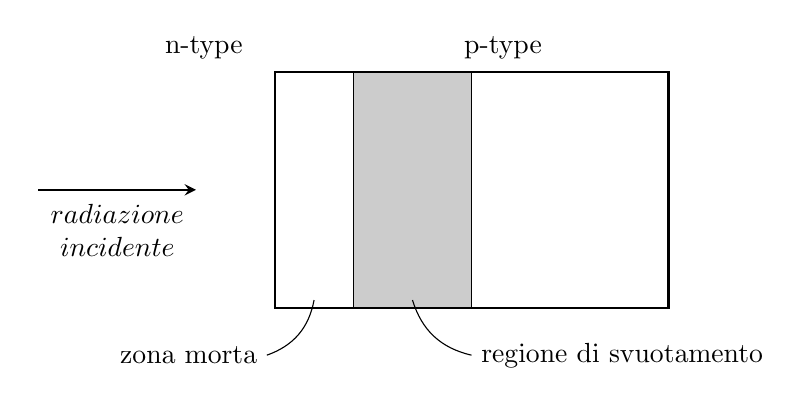
\begin{tikzpicture}
     \draw[fill=gray!40!] (1,-1.5) -- (1,1.5) -- (2.5,1.5) -- (2.5,-1.5) -- cycle;
      \draw[thick] (0,-1.5) -- (0,1.5) -- (5,1.5) -- (5,-1.5) -- cycle;
      \node at (-0.9,1.8) {n-type};
      \node at (2.9,1.8) {p-type};
      \draw[bend right] (-0.1,-2.1) node[left] {zona morta} to (0.5,-1.4);
      \draw[bend left] (2.5,-2.1) node[right] {regione di svuotamento} to (1.75,-1.4);
      \draw[thick,-stealth] (-3,0) -- (-1,0) node[midway,below]
      {$\begin{array}{c}
       \text{radiazione}\\
       \text{incidente}
       \end{array}$};
   \end{tikzpicture}
 \end{figure}
Tuttavia, il principale problema di questo tipo di rivelatori è che la giunzione non si forma in superficie, bensì si forma a una profondità di alcune decine di micron. Questo vuol dire che una particella che incide sul rivelatore dovrà attraversare prima una zona che per i nostri scopi è una zona morta, perché non è una zona utile per la rivelazione, per poi entrare nella regione di svuotamento. Ciò comporta una perdita dell'informazione trasportata dalla particella, il che limita le misure di energia. Tale fattore costituisce il principale svantaggio, inoltre un altro svantaggio sono le alte temperature che si adoperano, perché aumentano il rumore e tendono a diminuire la vita media dei portatori di carica, rendendo più difficile la loro misura. I vantaggi sono la robustezza e le basse contaminazioni superficiali.

\subsection{Rivelatori a barriera superficiale (SSB)}
Il problema della barriera a una certa profondità, dunque della presenza di una zona morta viene superato dai rivelatori a barriera superficiale. Questi sono basati su dei diodi Schottky, cioè dei diodi che si formano, anziché con due semiconduttore, con un semiconduttore e un metallo.
\begin{figure}[H]
   \centering
   \includegraphics[width=0.9\textwidth]{immagini/rivelatori_a_barriera_superficiale.png}
\end{figure}
Quando infatti andiamo ad accostare un metallo con un semiconduttore, quello che succede è la formazione anche in questo caso di un aggiunzione. Solitamente si adopera dell'oro su un materiale di tipo n o dell'alluminio su un materiale di tipo p.

La produzione di questi rivelatori avviene innanzitutto trattando la superficie chimicamente, ossidandola e poi depositando lo strato metallico per evaporazione. Il tutto infine viene montato su un anello isolante con delle superfici metallizzate per assicurare il contatto elettrico.

\begin{minipage}{0.49\textwidth}
   \begin{figure}[H]
      \centering
      \includegraphics[width=0.9\textwidth]{immagini/schema_rivelatore_SSB.png}
   \end{figure}
\end{minipage}
\begin{minipage}{0.5\textwidth}
   \vspace{0.4cm}Il rivelatore che adoperiamo per l'esperienza della misura della radiazione $\alpha$ è di questa tipologia e si presenta così come mostrato nella figura accanto.
   
   L'esterno è l'anello su cui viene montato il tutto, mentre all'interno è posizionato il rivelatore che è una fetta di silicio. Il connettore ad avvitare permette infine il passaggio del segnale.
\end{minipage}

\vspace{0.3cm}Vediamo i vantaggi di questa tipologia di rivelatori:
\begin{itemize}[leftmargin=0.5cm]
   \item In questo caso abbiamo dei rivelatori totalmente svuotati, per cui non abbiamo nessuna zona morta come avveniva invece nel caso precedente;
   \item Possono essere profondi anche diversi millimetri. Nel nostro caso non ci interessa, però potrebbe essere utile per la rivelazione di altre particelle;
   \item Il processo di lavorazione avviene a temperatura ambiente, a differenza di quanto visto per i rivelatori a diffusione.
\end{itemize}
Per quanto riguarda gli svantaggi:
\begin{itemize}[leftmargin=0.5cm]
   \item Lo strato metallico depositato è così sottile che purtroppo non isola dalla luce, quindi sono rivelatori che possono essere sensibili alla luce. Infatti i fotoni del visibile hanno un'energia sufficiente a poter creare delle coppie elettrone-lacuna;
   \item Sono anche sensibili a possibili contaminazioni superficiali.
\end{itemize}

\subsection{Ion-Implanted Diodes}
Altre tipologie di rivelatori si basano invece sull'utilizzo dell'impiantazione ionica, in il drogaggio viene realizzato attraverso l'utilizzo di acceleratori che accelerano dei fasci di ioni, che sono le nostre impurità, per impiantarli all'interno di un materiale semiconduttore. \E un processo violento essendo sostanzialmente un bombardamento del materiale semiconduttore, e questo fa sì che alla fine sia necessario un annealing a $500 \, \rm ^{\circ}C$ per poter ripristinare i danni eventualmente causati da questo processo di impiantazione.

Per quanto riguarda i vantaggi, essi sono dei rivelatori molto stabili e con finestre di ingresso molto sottili, quindi con zona morta di poche decine di nanometri, ma lo svantaggio è che sono parecchio costosi, soprattutto per i processi di produzione che richiedono l'utilizzo di un acceleratore. 

\subsection{Rivelatori a deriva di litio Si(Li)}
L'ultima categoria di rivelatori che introduciamo sono i rivelatori a deriva di Litio, i quali cercano di risolvere il problema delle piccole dimensioni della regione di svuotamento, infatti abbiamo detto che c'è sempre un limite alle dimensioni di questa regione, perché poi il diodo va in rottura. Per risolvere questo problema si utilizza una cosiddetta aggiunzione p-i-n, dove al materiale di tipo p e al materiale di tipo n si frappone un materiale di tipo compensato. In questo modo è possibile ampliare la zona in cui può avvenire la rivelazione, potendo arrivare anche a spessori di $10-15$ mm, il che è molto utile laddove abbiamo bisogno di range elevati per poter fermare una particella e misurarne l'energia.

Vediamo il processo con cui avviene la realizzazione di questi rivelatori:
\begin{figure}[H]
   \centering
   \includegraphics[width=\textwidth]{immagini/rivelatore_a_deriva_di_litio.png}
\end{figure}
Il litio viene posizionato sulla superficie di un materiale drogato di tipo p, viene fatto diffondere attraverso l'applicazione di un campo elettrico e alla fine quello che si ottiene è un'aggiunzione di tipo p-i-n, in quanto a sinistra rimane la zona p perché il litio non è arrivato fino a questa estremità, la regione centrale diventa di tipo compensato, perché era drogata di tipo p e ad essa aggiungiamo il litio che è di tipo n e infine a destra rimane la zona di tipo n dovuta essenzialmente a un'alta concentrazione di litio.

I vantaggi sono dovuti a questi spessori elevati, che fanno sì che vengano utilizzati per la spettroscopia beta o per i raggi X a bassa energia. Gli svantaggi sono invece il fatto che si debbano adoperare a temperature basse a causa dell'elevato rumore termico, inoltre anche la conservazione dovrebbe avvenire a temperatura basse per mantenere inalterata la zona intrinseca.

\subsection{Realizzazione contatti}
L'ultimo aspetto che discutiamo sul rivelatore al silicio riguarda la realizzazione dei contatti. 

Non è possibile creare un contatto ohmico utilizzando un materiale metallico sul semiconduttore perché quello che si viene a creare è un diodo Schottky, quindi un ulteriore giunzione e dunque un ulteriore regione di svuotamento, che non è ciò che desideriamo. Quello che allora si fa prima di applicare un contatto metallico è realizzare una regione altamente drogata, ad esempio nella figura seguente possiamo vedere una regione di tipo n+ prima del contatto metallico.
\begin{figure}[H]
   \centering
   \includegraphics[width=0.5\textwidth]{immagini/realizzazione_contatti.png}
\end{figure}

\section{Caratteristiche dei rivelatori a semiconduttore}

\subsection{Linearità}
In ogni rivelatore che misura l'energia, ci aspettiamo un ottimo grado di linearità, per cui se arriva una particella con un'energia $E$ ci aspettiamo che il segnale prodotto sia proporzionale a tale energia, in maniera tale da avere una risposta lineare. Nel caso di un rivelatore a semiconduttore, se questo ha uno spessore sufficiente ad arrestare la particella al suo interno e quindi a misurare tutta l'energia, ci aspettiamo che il segnale in tensione che viene indotto sia proporzionale alla carica prodotta, quindi alle coppie elettrone-lacuna che sono state create a seguito della perdita di energia della particella all'interno del rivelatore, diviso la capacità, in quanto il diodo non è altro che un condensatore a causa della sua configurazione elettrica.

Se la radiazione ha energia $E$, allora dovrebbero essere create $E/w$ coppie elettrone-lacuna, dove $w$ è l'energia media per creare una coppia. In generale però il rivelatore avrà un'efficienza di raccolta $\eta$, che indica il fatto che non tutte le coppie prodotte potrebbero essere raccolte, dunque soltanto una carica $Q=\eta E/w$ e quindi il segnale misurato sarà dato da
\begin{equation*}
   V
   =\frac{Q}{C}
   =\eta \frac{E}{w C}
\end{equation*}
Il fatto che purtroppo perdiamo alcune coppie non ci spaventa, in quanto ciò che conta è che si mantenga la linearità tra il segnale prodotto e l'energia depositata nel rivelatore.

In generale, la risposta dei semiconduttori è abbastanza indipendente dal tipo di particella, quindi se entra un elettrone o se entra una particella alfa, normalmente se si deposita la stessa energia viene prodotto lo stesso segnale. Tale discorso è valido fintanto che non si considera l'arrivo di ioni: in tal caso di si generano degli effetti di plasma, quindi delle nuvole di elettroni particolarmente dense che vanno a distorcere il campo elettrico all'interno del rivelatore e pertanto la linearità non è del tutto assicurata.

Nel caso in cui invece il rivelatore non sia sufficientemente spesso, viene misurata semplicemente una perdita di energia, quindi a volte i rivelatori a semiconduttore vengono utilizzati come rivelatori di trasparenza, cioè con lo scopo di essere attraversati e far perdere alle particelle una quantità di energia molto piccola. In questo caso la risposta non è lineare con l'energia della particella.

\comment{

\textbf{continua a 1:06:30 circa}

\subsection{Risoluzione in energia}
La risoluzione di questi rivelatori è tipicamente abbastanza buona. Infatti servono pochi elettronVolt per generare una coppia elettrone-lacuna, a differenza dei valori di energia media per creare una coppia ione-elettrone in un rivelatore a gas che sono dell'ordine di $20-40$ eV. La conseguenza di ciò è che, a parità di energia depositata, nel caso di un rivelatore al silicio si produce un numero di coppie che è 10 volte superiore rispetto a quanto si produrrebbe in un rivelatore a gas, e il fatto di avere un numero di coppie elevato fa sì che la risoluzione sia migliore.

\E chiaro che l'energia necessaria a creare una coppia dipende dal gap di energia proibita. Ad esempio, alla temperatura di 77 K per il silicio sono necessarie energie dell'ordine di $3-4$ eV letto, mentre per il germanio poco meno di 3 eV. Precisiamo che queste sono in realtà le energie per produrre una coppia, mentre le energie del gap sono in realtà più piccole. Ciò è legato al fatto che due terzi dell'energia vengono spesi per creare delle vibrazioni reticolari. Quindi ci ritroviamo ad avere bisogno di almeno 3-4 letto molto per creare una coppia.

Quando vogliamo misurare l'energia, l'energia che noi misuriamo in realtà la misuriamo in termini del numero $n$ di coppie che si generano. Tale numero è dato dal rapporto tra l'energia $E$ che viene depositata nel rivelatore diviso $w$, che è l'energia media per creare una coppia. Abbiamo detto questo vale sia per i rivelatori a gas che per i rivelatori al silice, con l'unica differenza che nei rivelatori a gas $w$ è dell'ordine all'incirca di 30 eV mentre nel rivelatore a semiconduttore $w$ è dell'ordine di circa 3 eV, quindi circa un decimo. Più precisamente, quando diciamo che il numero di coppia è $n$ stiamo parlando di un valore medio $\bar{n}$, perché sebbene sia vero che si producono queste coppie poi le coppie che danno luogo al segnale sono una parte perché avvengono diversi fenomeni di fluttuazioni statistiche e quindi il numero $\bar{n}$ che misuriamo e che è indice della mia energia in realtà può variare da evento a evento, quindi ad esempio se io invio il rivelatore al silice delle particelle alfa come quello che vi troverete a fare a breve elaboratorio di 5 MeV, questi 5 MeV vengono persi nel rivelatore e deranno luogo a un certo numero di coppie che produrranno il segnale, ma questo numero di coppie fluttua ovviamente a seguito di fenomeni in natura sadistica e quindi quando io dico che sono andando a misurare lo spettro in energia e le particelle alfa e trovo un picco molto stretto come quello in figura, questo rappresenta il numero di particelle alfa che hanno una certa energia. Ora quello che io riporto sull'asse orizzontale, l'energia, in realtà equivale a N, equivale a dir a quante cariche, quante coppie ho generato e quindi il fatto di non avere una delta di dirac come io mi dovrei aspettare perché sto mandando 5 MeV, mi dovrei, dovrei trovare sempre 5 MeV, in realtà trovo a volte dei valori un po' più grandi a volte un po' più piccoli per quale motivo perché ci sono delle flutuzioni dovute proprio al numero di coppie che creano il segnale, questo numero fluttua, coccilla leggermente quindi è come dire che quello che gli osservo solo spettro in energia è una conseguenza del numero di coppie N che ogni volta si producono e che vengono raccolte che non sono sempre le stesse. Quindi posso valutar un N medio, quindi dalla formula che abbiamo visto prima ma poi rispetto a questo N meglio ogni volta ho delle fluttuazioni. La risoluzione di energia come viene valutata, se vado a ricordare, andando a guardare il picco e studiandone la larghezza, in particolare mi concentro sulla larghezza a metà altezza, quindi se questo ad esempio è il massimo del picco vado a considerare la metà altezza, quindi il massimo diviso 2 e vado a vedere la larghezza del picco a metà altezza, quella che è indicata normalmente con la sigla FWHM Full Width At Alph Maximum. La risoluzione in energia la possiamo indicare con R e data dalla larghezza a metà altezza diviso l'energia, possiamo moltibricarla per 100, per averla in percentuale però questa è la formula. Se il picco ha una forma gaussiana si può dimostrare che questa larghezza a metà altezza è all'incirca 2,35 per la deviazione standard della gaussiana diviso l'energia. Quindi se abbiamo una gaussiana siete agevolati perché ad esempio possiamo realizzare un best fit della vostra distribuzione con una funzione gaussiana e strare il parametro sigma che rappresenta la deviazione standard e utilizzarlo per valutarla la larghezza a metà altezza semplicemente moltirricando per 2,35. Altrimenti l'alternative è guardare la distribuzione dei valori che abbiamo misurato, guardare la larghezza a metà altezza materialmente come abbiamo fatto qui adesso. Allora come mettiamo in relazione la risoluzione al numero di coppia? Abbiamo detto abbiamo questa relazione che abbiamo scritto qui in alto n medio uguale ae su w quindi quando vado a riscrivere la risoluzione al denominatore posso andare a sostituire ae il numero n per w. Al numeratore mi riscrivo 2,35 per come sigma? Sigma è la deviazione standard di questa distribuzione che posso immaginare appunto essere anch'essa legata alla sigma della distribuzione del numero di coppia quindi posso andare a scrivere che sigma con n non è altro che sigma con e diviso w. Andando quindi a sostituire questo diventa w per sigma con n, w e w posso semplificare e quindi la mia risoluzione banalmente la posso andare a scrivere la scrivo qua sotto r come 2,35 sigma con n diviso n. Quindi ho riscritto banalmente la risoluzione in termine di n numero di coppia quindi la risoluzione sarà dato dalla larghezza di questa distribuzione del numero di coppia su numero medio di coppia generato. Se la distribuzione, dato che stiamo parlando di numero di coppia, la distribuzione che regola la produzione di queste coppia, la distribuzione di tipo possaniana, posso approssimare sigma alla radice di n e quindi capite che questo diventa 2,35 radice di n su n. Quindi se canciglie un attimo, andiamo a fare il calcolo per i due casi. Quindi r l'abbiamo scritto come 2,35, 1 su radice di n. E allora ad esempio se nel selicio si producono, abbiamo detto in media, 10 volte in più di coppia, capite che la risoluzione non rivoluta alla selicio sarà dato da 2,35 diviso 1 sulla radice di 10n. E quindi sostanzialmente vedete c'è un fattore all'incirca un terzo, quindi la risoluzione di un rivelatore alla selicio è all'incirca un terzo rispetto alla risoluzione di un rivelatore a grassa. Suffizialmente per il fatto che si producono un fattore di 10 in più di coppia. Quindi dire che è un terzo vuol dire che è più piccolo e quindi vuol dire che ovviamente è una risoluzione migliore. Nei rivolatori al selicio si possono raggiungere anche le risoluzioni dell'1\% e 

anche più bassa volta, dipende dal modo di operare. Ci sono domande su questi passaggi. Sensibilità ed efficienza in trince. In trince che ha di un rivelatore a semiconduttore è dell'ordina del 100\%. Vi ricordate cos'è l'efficienza in trince che rappresenta il rapporto tra il numero di particelle che hanno dato l'uogo a un segnale diviso il numero di particelle incidenti. Quindi arriva una particella, incide sul rivelatore, perde energia. Questo da luogo a un segnale rivolabile non è detto, in questo caso sì, praticamente prossima al 100\%. In altri rivolatori l'efficienza in trince dovrebbe essere più bassa anche a secondo del tipo di particella. Quali sono i limiti? I limiti potrebbero essere la presenza di una soglia minima necessaria sul segnale da rivelare. Legato al fatto che comunque sì e ci sono delle correnti di dispersione e l'elettronica che introducono un minimo di rumore. Quindi possono creare dei segnali che in realtà sono segnali di rumore. Sono segnali ovviamente di bassa ampiezza. Questo fa sì che se non vogliono essere confusi con segnali fisici devono essere in qualche modo discriminati, cioè eliminati dell'acquisizione. Questo può essere fatto imponendo una soglia minima al di sotto della quale non rivelare nulla, non acquisire nulla. Quindi questo però da un lato ovviamente vi aiuta a eliminare il rumore. Dall'altro però vi potrebbe far perdere qualche segnale fisico di interesse, quindi abbassare leggermente l'efficienza in trincega. La presenza di una zona morta potrebbe anche qui imporre una certa perdita nell'efficienza perché magari i particelli di bassa energia riescono ad attraversare la zona morte, quindi non vengono misurate. Quindi hanno inciso sul rivelatore ma non sono state misurate. La densità, vi dicevo questo è un vantaggio perché permette di avere un elevato stopping power. Ad esempio guardate qui in questo grafico, come non è facilmente leggibile a causa del della qualità. Viene riportata l'energia della particella da 1 a 100 membo e sulla sé verticale viene riportato il range in micron e i grafici che vedete qui le linee corrispondono a diverse tipologie di particelle, protone ed autoni, trizzi, ediotree e alfa. Concentriamoci ad esempio sulla situazione di terci e di troveremmo il laboratorio, quindi i particelle e l'alfa da 5 Mav che incidono sul sidicio. Questo grafico ci permette di capire che spessore deve avere il rivelatore per assicurarci che tutta l'energia venga persa all'interno del rivelatore. Ad esempio a alfa da 5 Mav ci ritroviamo qui grosso modo, vedete che siamo a range dell'ordine della ventina di micron e quindi è sufficiente un rivelatore di questo spessore per poter far sì che le particelle alfa perdano tutta la loro energia. Questo vi dicevo è un vantaggio perché sono necessari spessori veramente ridotti, quindi rivelatori compatti per poter andare a misurare energia di particelle anche molto energetiche. Infine, un'ultima qualità di questi rivelatori che abbiamo una diffusione estremamente più bassa, più piccola rispetto a quelle rivelatori a gas, si fa sì che questi rivelatori possono essere utilizzati più facilmente come rivelatori di posizione, quindi per andare a misurare la posizione della particelle incidente.

Il tempo di risposta, vi ho detto, sono rivelatori molto veloci in generale possono essere utilizzati come rivelatori di timing certamente molto più performanti rispetto ai classici rivelatori a gas. Tipicamente i tempi di salidità di un segnale sono dell'ordine dei nano secondi quindi estremamente veloci. Altre rivelatori veloci che avevamo visto erano ad esempio gli scintillatori, se vi ricordate abbiamo fatto qualche misura lo sceloscopio. Un problema però di questi rivelatori è il cosiddetto danneggiamento a rada raviazione, cioè cosa succede se questi rivelatori vengono esposti a notevoli dosi di raviazione. Purtroppo questo avviene soprattutto in alcuni ambienti quando possono essere appunto gli esperimenti sotto fascio, sotto accederatore o esperimenti nello spazio e questo modifica le qualità e le proprietà del rivelatore. In generale i danni che si possono creare sono di due diversi tipi, possono essere o danni del bike, cioè proprio del corpo, della massa che costituisce leaponduttore oppure dei danni sulla superficie, quindi sull'ossido che normalmente rivesse questi rivelatori. Gli effetti sul bike appunto sono effetti che si manifestano come danneggiamento al arreticolo e in generale sono dovuti alle cosiddette radiazioni nile cioè radiazioni non ionizzanti. Cosa comporta poi ne satti concretamente che magari può cambiare l'attenzione di svuotamento. Quindi se ad esempio voi stavate lavorando con il vostro rivelatorio a 10 volt e attenevate determinate prestazioni, vi rendete conto che a seguito di questo deneggamento non sono più sufficienti 10 volt, ma dovete doverare 12 volt, 15 volt. Quindi cambia la vostra attenzione di lavoro a cui ottenevate un buon svuotamento della regione. Potrebbe aumentare la corrente. Quindi una corrente che comporta un rumore e quindi questo potrebbe richiedermi l'utilizzo di un raffreddamento, oppure diminuire l'efficienza nella raccolta della carica. Qui ad esempio possiamo vedere come cambia l'attenzione di lavoro man mano che aumenta la dose. Questi sono dei dati sperimentali realizzati su un determinato tipo di rivelatore. Vedete come l'attenzione di lavoro man mano cambia. L'importante è ovviamente studiare per bene i possibili deneggiamenti di radiazione. Questo è una parte importante di quello che costituisce hierarchica la progettazione di un esperimento. Ad esempio tutti gli esperimenti acceleratori come può essere l'HCO o altri acceleratori richiedono anni e anni di progettazione anche per studiare questi effetti. Perché sono arrivelatori che ovviamente richiedono lo sforzo di anni di lavoro e devono operare per almeno 5, 10 anni. quindi bisogna assicurarsi che il rivalatore non subnisca un deterioramento eccessivo e che quindi possa lavorare per l'intervallo di tempo in cui dovrebbe lavorare. Quindi spesso la tecnologia non esiste nel momento in cui si immagina di dover costruire il rivalatore, quindi si lavora per costruire e arrivare a questi obiettivi. Gli effetti sulla superficie invece sono tipicamente dovuti a radiazione ionizzante e questo comporta sostanzialmente la presenza di cariche positive che si accumulano sugli ossidi e poi può anche influire sull'umore e sulla tensione di rottura. Gli effetti che vengono prodotti dal deneggiamento e da radiazione possono essere o effetti cumulativi che si vanno sommando nel tempo e sono dei danni che non si possono riparare, sono dute proprio all'esposizione prolungata alla radiazione che è un po' quello che vi ho descritto prima, ha immaginato il rivalatore deve essere adoperato in un esperimento sotto fascio, chiaramente è un accumulo costante nel tempo che comporta ovviamente dei danni irreparabili oppure possono verificarsi e questi si studiano pure degli eventi singoli che possono essere proprio o eventi transitori, immaginate ad esempio banalmente il cambio di un bit da 0 a 1 questo potrebbe essere un effetto transitorio o eventi catastrofici permanenti ma questi sono singoli eventi quindi che potrebbero accadere oggi come tra 10 anni quindi non sono legati proprio a un acuno come abbiamo visto nel caso precedente ragazzi mi fermerei qui oggi e riprendiamo questa parte la prossima volta quindi sono ormai soltanto applicazioni del rivalatore a ciricio e parleremo poi del introdurro una delle esperienze che farete quella appunto un rivalatore a ciricio e particelle alfa e parleremo delle tecniche di vuoto perché appunto quando adopererete questo rivelatore dovrete lavorare con una cameretta da vuoto quindi introdurremo qualche concetto di questo tipo allora noi ci vediamo giovedì pomeriggio mi sembra in aula e mi sbaglio ci hanno spostati allora ragazzi qua interrompo la registrazione e ci vediamo giovedì

\textbf{lez 15}

\vspace{4cm}

Allora ragazzi, riprendiamo quello che avevamo iniziato la volta scorsa. Se vi ricordate avevamo in prodotto i rivelatori a semiconduttore, era l'ultima tipologia di rivelatori che affrontiamo in questo corso. Vi ricordo molto molto velocemente la struttura di base di un rivelatore a semiconduttore e vi ricordo che si basa su un'aggiunzione PN, quindi quindi realizzata con un materiale semiconduttore drogato di tipo N e accanto un materiale drogato di tipo P. In questo questo è possibile realizzare nella zona dell'aggiunzione una regione di svuotamento che è una regione priva di cariche libere. Invece sono presenti delle cariche fisse che sono i milioni presenti nel nerreticolo che generano una potenziale, detto potenziale di contatto. Quindi vedete qui ad esempio la forma del campo elettrico proprio in corrispondenza della giunzione e qui come vengono deformate le bande energetiche dei materiali. Questa è una regione che si è adatta bene allo scopo della rivelazione perché nel momento in cui dovesse passare una particella e depositare dell'energia questa energia verrà utilizzata per produrre nuove coppie elettrone e lacuna, chiaramente il numero di coppie proporzionale all'energia che viene depositata nel materiale e queste coppie possono essere raccolte proprio grazie a questa differenza di potenziale. Chiaramente poi è necessario andare a mettere degli elettrodi per poter raccogliere la tarica, tuttavia essendo un potenziale molto piccolo la regione di svuotamento comunque molto ridotta e quindi per aumentarla quello che si fa è polarizzare inversamente l'aggiunzione e quindi andare ad applicare un potenziale positivo dalla parte n è un potenziale negativo del lado p. In questo modo la regione di svuotamento aumenta e diventa ovviamente una regione ancora più adatta alla rivelazione. Tante volte questi rivelatori semi-conduttore vengono utilizzati per misurare radiazione alfa che viene arrestata in poche decine di micron e quindi in realtà queste giunzioni non devono avere delle regioni di svuotamento particolarmente stesse, però per la rivelazione di altre radiazioni come ad esempio gli x, le regioni anche dell'ordine del millimetro e quindi abbiamo visto anche delle tecniche costruttive di realizzazione di questi rivelatori per arrivare a estensioni dell'ordine dei millimetri. Avevamo concluso un po' tutta questa parte, eravamo arrivati anche a discutere le caratteristiche di questi rivelatori al silicio e il danneggiamento della radiazione e dovevamo concludere questo argomento parlando delle applicazioni nella spettroscopia di particelle cariche. Questi rivelatori hanno delle proprietà molto positive, abbiamo detto hanno una risposta temporale abbastanza pronta, abbastanza veloce quindi sono adatti ad esempio per applicazioni di timing, dove volete andare a misurare delle differenze di tempo tra segnali elettrici, quindi forniti ovviamente da rivelatori. La risoluzione è ottimale, stiamo parlando di risoluzioni dell'ordine dell'1\%, quindi molto più bassa rispetto a quelle che abbiamo visto con altre tipologie di rivelatori e quindi proprio per queste proprietà questi rivelatori venivano utilizzati nel campo della spettroscopia di particelle cariche. Inoltre sono disponibili come abbiamo detto in un'ampia varietà sia di spessori che anche di area sensibile, hanno un'efficienza prossima al 100\% nel caso di protoni, particelle alfa ma anche ioni pesanti e di ricevo che lo spessore da doperare chiaramente si deve valutare in base all'applicazione, quindi in base al tipo di particella che si vuole andare a parlare in base anche alla sua energia. E proprio per questo motivo nel campo della fisica moderna, più che fisica moderna della fisica attuale, soprattutto fisica delle alte energie, questi rivelatori vengono utilizzati ampiamente, hanno appunto le prestazioni proprio adatte per andare ad affrontare anche degli ambienti spavorevoli, come ambienti in cui si ha una elevata dose di radiazione, una elevata densità di particelle e quindi negli ultimi decenni ci sono stati enormi sviluppi soprattutto in questo campo con ovviamente ritadute poi in altre tipologie di applicazioni come ad esempio il campo della medicina, quindi tante volte alcune tecnologie si sviluppano nel campo della ricerca e poi vengono trasferite in automatico nel campo, in altri tipi di campo, campo arespaziale, campo della medicina. Un altro vantaggio di questi rivelatori è che spesso è utile avere dei rivelatori molto subtili, vi ho detto che questi rivelatori possono essere adoperati anche come rivelatori in trasparenza, vengono attraversati della particella, viene effettivamente depositata dell'energia, ma questa energia è molto piccola, quindi è come se fosse una piccola perturbazione effettivamente del percorso e della particella nelle sue proprietà. E questo è un vantaggio perché da un lato abbiamo comunque sia un segnale che mi indica il fatto che è passato una particella e quindi eventualmente per problematiche di tracciamento di tracking, quindi sapere attraverso quali punti la particella è passata è utile avere questi rivelatori perché sono in grado proprio di misurare la posizione della particella senza perturbarne eccessivamente le caratteristiche. Quindi ormai tutti, quasi tutti gli esperimenti di alta energia e nello spazio utilizzano ampiamente questi rivelatori al silicio. Questo è un grafico che ormai è un po' datato perché insomma risale ormai quasi a vent'anni fa, però era giusto per darvi un'idea vent'anni fa di quali erano gli esperimenti che tipicamente utilizzavano rivelatori in questo caso al silicio di tecnologia strip, ora vi dirò un po' qualcosa qualcosa questa tecnologia. Comunque al di là di questo dettaglio vedete colorati le diverse applicazioni, questi sono acceleratori, quindi quindi verde e rosso si riferiscono a esperimenti prestoacceleratori e l'HC è l'acceleratore al momento più potente che riesce ad accelerare alle massime energie fino a la realizzata mentre in blu vengono riportati gli esperimenti nello spazio. Quindi vedete che appunto... ma che è questo rumore ragazzi? Sto riuscendo a favori. Ansì rispetto a qualche giorno fa, a qualche qualche di giorni fa. A inizio febbraio abbiamo fatto un esame del dottorato, un esame fino a il dottorato qui in quest'aula, è stato un inferno veramente, non si capiva niente. Comunque, vi dicevo, vedete appunto la varietà di applicazioni qui sotto sono riportati proprio nel dettaglio le sigle degli esperimenti che fanno uso di questa tecnologia al siri. Cioè, ad esempio, quello che mostra la maggiora utilizza, ad esempio l'esperimento CMS, non so se l'abbiamo mai seguito nominare, un esperimento presso l'acceleratore e l'HC. Diciamo uno dei esperimenti che ha contribuita alla scoperta del bosone X. E vedete qui il grafico riporta l'area in metri quadri. Quindi Quindi questo caso, vedete, CMS utilizza 214 metri quadri di rivelatori, in questo caso al siriscio in strippo. Ma altri rivelatori non sono da meno, comunque una tecnologia particolarmente utilizzata. Guardiamo ora un po' più più dettaglio alcune forme, alcuni rivelatori più moderni che utilizzano sempre la tecnologia basata sul siriscio. In generale, si possono avere due possibili scelte quando si vuole utilizzare il siriscio per ricostruire la posizione della particella. Quindi la particella incide sul rivelatore, voglio sapere esattamente in che punto è passata la particella. Allora, in questo caso si possono adoperare due scelte distinte. O si utilizza un readout continuo o un readout discreto. Capiremo ora la differenza. E in particolare faremo riferimento a queste tipologie di rivelatori al siriscio. I rivelatori a strip, che sono quelli di cui vi ho parlato nella slide precedente, quelli a pixel o pad e quelli a drift. Quindi vedete già un'immediata differenza, soltanto nella rappresentazione. Strip sta a indicare in inglese una striscia. E infatti vedete che qui questo rivelatore, ora andremo a vedere un po' più nel dettaglio, presenta queste strisce parallele, l'un all'altro, che prendono nel nome appunto di strip. Pixel o pad, ovviamente conoscete i pixel perché siete abituati ovviamente con le fotocamere, ecco qualcosa di similare anche in questo caso. Vedete una matrice di elementi che prendono nel nome appunto di pixel. Infine quelli drift vedete qui nuovamente una striscia a strip, però evidentemente c'è qualche differenza a rispetto al caso delle strip. E a seconda del tipo di rivelatore avremo un readout continuo o un readout discreto. 

Partiamo ad esempio a rivelatori a strip o micro strip quando queste strip hanno dimensioni di pochi micron. Allora vediamo un po' la struttura di questo rivelatore. Si basa tutto sempre su giunzioni piene quindi non è qualcosa di totalmente diverso da quello che abbiamo fatto fino ad esso. Però in più si sfrutta il fatto di poter realizzare gli elettrodi con determinate geometrie. Quindi qui la caratteristica è che gli elettrodi di lettura sono costituiti da queste strip che vengono posizionati parallelamente, l'un all'altro ha una distanza opportuna tipicamente della decina di micron. Il segnale che viene prodotto all'interno del rivelatore induce il segnale sull'elettrodi lettura e chiaramente andrà in dur, il segnale sull'elettrodi più vicino. Quindi in base a dove passa la particella, ad esempio guardate questa linea che rappresenta una particella che è attraversata il rivelatore, qui questa particella avrà prodotto un certo numero di coppie elettrone e lacuna che migliano verso gli elettrodi inducendo un segnale ed è chiaro che la strip che viene interessata ci fornirà la coordinata spaziale, cioè il punto attraverso cui è passata la particella. Chiaramente è un'informazione monodimensionale perché l'unica informazione che abbiamo è lungo questa direzione. Quindi se viene colpita ad esempio il rivelatore al centro immagino che viene interessata la strip centrale se invece la particella colpisce il rivelatore più a sinistra sarà la strip di sinistra dal segnale e così via. Chiaramente qui vedete soltanto una porzione del rivelatore ma normalmente sono presenti centiraia di canali in base all'essenzione del rivelatore. Quindi questo rivelatore è diciamo di posizione in questo caso monodimensionale perché ci dà l'innicazione su una sola coordinata spaziale sul piano ovviamente. Poi il meccanismo, il principio di funzionamento è esattamente sempre lo stesso quello che abbiamo visto prima quindi sempre giunzioni pn polizzate. Se volessimo avere un'informazione bidimensionale sul piano cosa potremmo fare? Una tecnica che viene aggoperata è semplicemente andare a sovrapporre due strati di rivelatore a strip come vedete qui con una certa inclinazione ovviamente. Questo vi fornirà l'informazione bidimensionale grazie al fatto di conoscere le strip interessate su ciascun piano però può portare eventualmente a dei casi di ambiguità perché se passa una sola particella attraverso entrambi gli strati allora non c'è alcuna ambiguità perché verrà interessata una strip per piano ma se per caso simultaneamente come può avvenire ad esempio in un esperimento sotto fascio sono più particelle ad attraversare i due strati allora inevitabilmente si crea un'ambiguità. Guardate qui l'esempio riportato in basso a destra. I punti verdi sono i punti reali attraverso cui è passata la particella, sono passate due particelle simultaneamente allora in basso a questa posizione ora magari il grafico è piccolino però possiamo immaginare qual è la strip di ciascun strato interessato anzi ciascun strato avrà due strip interessate una per particella quindi nel momento in cui voglio risalire alla posizione devo andare a considerare tutte le possibili combinazioni di queste coppie di strip e quindi cosa succederà che ne ricostruirò due correttamente ma ce le saranno altre due che sono quelle segnate in rosso che sono diciamo legittime nel senso derivano proprio dalla combinazione delle strip colpite ma in realtà nascono insomma sono in realtà spuri non sono collegata al reale passaggio di particelle quindi è vero che è utile sono a porre questi strati di strip però bisogna stare attenti a questi casi di ambiguità quanto vale la risoluzione chiaramente la risoluzione spaziale quindi la capacità di ricostruire la precisione con cui si ricostruisceotomia la posizione dipende dalla distanza tra le strip più queste sono vicino tra di loro migliore sarà la risoluzione spaziale in particolare se vi ricordate già questo discorso l'avevamo fatto nel caso delle camera fili, qui è un discorso analogo, data la distanza tra due elettrodi, la risoluzione data da questa distanza diviso la radice di 12. Quindi se ad esempio la distanza è 20 micron, la risoluzione reale sarà 20 diviso la radice di 12. Questa è una conseguenza del teorema del limite centrale, dava un discorso durante il primo semestre. Quindi vedete una risoluzione molto spinta, si si arrivare anche a 5 micron, tempi di raccolta delle cariche molto veloci, anche decine di nanosecondi. Un unico difetto è questa eventuale ammiguità nella ricostruzione della posizione. E questo è un esempio di rivelatori al redout discreto, perché qui la posizione viene data grazie alla discretizzazione dell'elettrodo, cioè il fatto di avere tanti elettrodi separati. In un rivelatore ad drift invece abbiamo un redout continuo. Che cosa cambia rispetto a prima? In anzitutto il rivelatore ad drift fornisce entrambe le coordinate su un piano, quindi un'informazione bidimensionale. Come fa? La struttura sembra molto simile a quella strip. Vedete qui abbiamo sempre degli elettrodi che sono realizzati come strip, paralleli l'un all'altro. Ma queste in realtà hanno una funzione diversa rispetto a quella che abbiamo visto prima. Ciò che raccoglie il segnale sono in realtà questi anodi che vedete qui sotto forma di pad, cioè di piazzola. Andiamo a vedere cosa succede quando passa una particella in grado di produrre coppie elettroni di lacuna. Queste sono gli elettroni e le lacune che vengono prodotte, gli elettroni incominciano a migrare verso gli anodi grazie a una differenza di potenziale che viene realizzata attraverso queste strip. Quindi questo strip se vedete qui c'è un partitore di tensione. Questi strip vengono messe a potenziale evidentemente via via crescente in maniera tale che gli elettroni che si producono a seguito del rilascio di energia nel rivelatore, questi elettroni vengono guidati verso l'anodo. Quindi come facciamo ad avere la coordinata bidimensionale? Allora una coordinata che è quella lungo questo ass, penso che segue la manina del cursore, viene fornita da quale anodo è stato interessato, quindi quale anodo ha raccolto la carica. Evidentemente l'anodo più vicino raccoglierà la carica. L'altra coordinata questa, quella verso cui, lungo cui si muovono gli elettroni, viene fornita dal tempo di deriva, cioè da quanto tempo impiedono gli elettroni ad arrivare all'anodo. Capite che se la produzione di questi elettroni avviene qui a questa estremità, impiegaranno un certo tempo, se venisse invece in questa estremità gli elettroni arriverebbero subito, quindi il tempo di deriva sarebbe più piccolo. Quindi il tempo con cui questi elettroni derivano verso l'anodo ci fornisce la coordinata lungo questa direzione. Ecco che quindi abbiamo una informazione di natura bidimensionale. Sto vedendo che la risoluzione è completamente diversa. Io sono molto più allungata, voi vede tutto più compatto. Tuttavia qual è l'osvantaggio? Questi sono rivelatori più lenti perché bisogna aspettare una deriva che può essere anche abbastanza lunga degli elettroni e inoltre necessitano di temperature stabili. Questo è un esempio di rivelatore al redauto continuo perché a questo punto è vero che abbiamo una discretizzazione lungo questa direzione dovuta agli anodi, ma lungo è l'altra direzione. La lettura è continua, cioè questo tempo di deriva assume un valore che non è discreto, ma è continuo. È chiaro? Se ci sono domande interrompete. Vede qualcosa che è molto simile a un dispositivo che voi adoperate spesso. Il CCD, il Charged Couple Device, voi lo utilizzate spesso perché è l'elemento di base delle fotocamere. Anche questi CCD sono rivelatori al redauto continuo, si dicono anche rivelatori a memoria perché gli elettroni che vengono prodotti a seguito della ionizzazione non sono rimossi immediatamente, quindi non vengono raccolti immediatamente ad un elettrodo, ma vengono fatti passare, innanzitutto vengono confinati all'interno di un pixel e poi a poco a poco vengono fatti derivare fino alla raccolta finale, un po' come avviene qui, che gli elettroni vengono prodotti e poi man mano vengono fatti derivare. Ora vedremo che qualcosa di simile vale anche per i CCD. Vediamo proprio un'animazione che fa sia la cosa più semplice se fa per messerlo a questa. Niente, è peccato perché la vengono se clicco. Ah, perché funziona. Allora, vedete il CCD è costituito da la matrice di pixel, che sono questi quadratini che vedete. Questi pixel costituiscono righe e colonne. Quando viene attraversato, questo sensore viene attraversato in questo caso da luce, viene generata della carica e questa carica non viene raccolta immediatamente da un elettrodo, ma in realtà a seconda del punto in cui si è creata viene guidato lungo la colonna corrispondente. Quindi, su per esempio di trovarvi qui, la carica è stata prodotta qui grazie a un campo elettrico opportuno, quindi adere differenze di potenziale, è possibile guidare la carica prodotta da pixel a pixel fino ad arrivare a quest'ultima riga dove avviene la lettura. Quindi proprio grazie a questo sistema è possibile andare a risalire a quale pixel è interessato. Qui sotto vedete nel dettaglio proprio la fase di deriva. Questi sono i pixel di una colonna, vedete che inizialmente la carica è confinata qui dove si trova un potenziale positivo, dopo di che il potenziale positivo viene creato nel secondo pixel e azzerato nel primo, quindi in questo modo riuscite a far derivare le cariche fino all'ultima riga. I cct sono quindi rivelatori bidimensionale, vi viene fornita effettivamente la posizione in cui è venuta la rivelazione, hanno acuratezze spaziali anche molto elevate dell'ordine di 10 nigron, però hanno come difetto principale in un tempo di lettura molto lungo, quindi almeno hanno dell'ordine dei 10 mili secondi. E questo fa sì che questi rivelatori normalmente non possono essere adoperato nel campo della fisica delle alte energie perché sono troppo lenti. Succederebbe che ad esempio se pensiamo in un esperimento in un acceleratore ovviamente avvengono un certo numero di collisioni al secondo, se il rivelatore ancora è impegnato a misurare ciò che è avvenuto nell'evento precedente, succede il cosiddetto pile up, una sovrapposizione di eventi che chiaramente deve evitare. Quindi Quindi rivelatori non vengono adoperati in questo campo, ma vengono adoperati parecchio nel campo dell'astronomia. Hanno una bassa risoluzione energetica e spaziale, quindi vengono utilizzati nel caso dell'astronomia per spettroscopie di ragilis. Questo è un altro esempio giusto per farvi capire come vengono identificati i pixel interessati. Vedete, questa è una matrice piccolina di 4 x 3 pixel, anzi 3 x 3 per questo poi è la riga di rettura. Vedete incidono quattro fotoni che sono sostanzialmente quelli che colpiscono i pixel sottostanti, se vedete qui vedete i pixel interessati. Si produce in ciascuna di queste regioni la carica e questa carica ovviamente lungo ogni colonna viene fatta migrare verso la riga di rettura e alla fine quello che succede è che si ricostruiscono i pixel che sono stati effettivamente interessati nella radiazione per andare a ricostruire l'immagine. Chiaramente questo è un esempio esempio di 3 x 3 ma dovete immaginare matrici con milioni di pixel. Funziano in maniera analoga i cosiddetti rivelatori a pixel, quindi quelli sono i ccd. Ora vediamo invece nel caso della fisica nucleare cosa possiamo usare di analogo che sia però molto più veloce rispetto a un ccd. In questo caso noi adoperiamo il rivelatorio a pixel anche si costituiti da matrici di pixel che possono essere anche dell'ordine delle centinaia di milioni compressivamente a seconda della superficie da rivestire e quindi sono ovviamente dei canali indipendenti. Qui ritorniamo a un caso di redout discreto quindi ognuno è come se fosse un rivelatore indipendente dall'altro. Le dimensioni di queste pixel ovviamente capite che più sono piccole migliore sarà la risoluzione spaziale del mio rivelatore. Ormai si è arrivato anche a pixel dell'ordine di 15-20 micron di lato, quindi veramente piccoli. Sono rivelatori bidimensionali perché viene fornita sia la coordinata x che la coordinata y. Vi dicevo ormai abbiamo dimensioni particolarmente spinte dell'ordine delle poche decine di micron. Sono rivelatori che hanno un livello di rumore molto basso, il il dipende dalla capacità di questi rivelatori e quindi un buon rapporto segnale sul rumore. Cioè vuol dire che quando vengono attraversati da una radiazione si produce una carica quindi un segnale che si sopraeleva rispetto al fondo, quindi il rapporto segnale sul rumore è ottimale. Sono rivelatori veloci e sono particolarmente adatti nel caso di alte densità di particelle. Quindi immaginate di avere una situazione in cui abbiamo tante particelle l'una vicino all'altra, ma le volete distinguere e rivelare indipendentemente. Quindi la probabilità che due particelle cadano in un 

pixel di dimensioni così piccole è veramente remota, veramente bassa. Ecco perché questi rivelatori normalmente vengono posizionati nella regione a più alta densità. Quindi se immaginate un esperimento, un collider dove avviene un'interazione tra fasci, una contro l'altra, capite che è la zona più vicina alla collisione, al punto di collisione sarà quella con la più più densità di particelle. Più vi allontanate, più avere rivelatori così discreti non è necessario. Quindi tipicamente rivelatori al silizio non sono posizionati proprio all'inizio in prossimità della collisione. quali sono gli svantaggi ovviamente. Capite che abbiamo un numero di canali enormi da leggere? Ora vedremo un esempio concreto, giusto per rendersci conto di che numero li stiamo parlando. In lì è di principio ogni rivelatore ha bisogno di un connettore e di un cavo. Se parliamo di un rivelatore macroscopico, immaginate ad esempio il rivelatore che abbiamo utilizzato, lo scintillatore, col fotomultiplicatore. Dal fotomultiplicatore usciva un cavetto che trasportava il segnale. Ora immaginate di doverlo fare per miliardi di pixel di queste dimensioni. L'ansi è tutto già realizzare un filo di quelle dimensioni capite che diventano un problema, ma ora lo discuteremo, chiaramente una sfida tecnologica. Qui se vedete un ingrandimento di quello che è un rivelatore a pixel, questo è una matrice e qua sotto non so se riuscire a riferli. Sono dei piccoli fili microscopici che sono dei bonding, c'è proprio delle connessioni che vengono realizzate con delle opportune macchine, perché non si possono realizzare a mano, ma si realizzano con delle macchine, si chiamano bondatrici e vanno a realizzare come se fosse un filo però di natura microscopica, quindi dal rivelatore verso l'elettronica. Sono ovviamente molto fragili e richiedono tecnologia all'avanguardia. Perché? Perché innanzitutto il primo problema è vi dicevo quello di trasportare questo segnale fuori da ciascun pixel e allora come si fa? Capite ogni pixel è un rivelatore a 60, quindi ad esempio se il segnale che fu riesce da questo rivelatore ha bisogno di un'opportuna catena elettronica, questa catena elettronica dovrebbe essere replicata per tutti i pixel. E quello che si fa normalmente, che si faceva tempo addietro, ora questa è una tecnologia che si sta superando, era quella di realizzare l'elettronica, ovviamente sempre su strade di silicio, miniaturizzata e delle stesse dimensioni dei pixel. Vete quindi si aveva sostanzialmente una matrice di pixel che erano i rivelatori e sotto una matrice con la corrispondente elettronica. Come si fa la connessione si realizzava attraverso la tecnica che prende il nome di bump bonding, cioè un bonding non realizzato con un filo, ben sì con una pallina, come la vedete qui. Qui sotto abbiamo il sensore, qui sopra abbiamo l'elettronica, questa pallina di materiale conduttore costituisceurasse il contatto. Chiaramente la corrispondenza deve essere esatta di sensore e di pixel di elettronica. Il tutto viene a temperatura controllata perché comunque questa è una sorta di non dico stagno ma comunque un materiale che si deve sciogliere deve realizzare un contatto stabile e tuttavia questa tecnica aveva grossi difetti. Qui vedete degli ingrandimenti con il microscopio, per farvi rendere al conto della forma di questi contatti. Tuttavia aveva dei difetti enormi, un'efficienza estremamente bassa quindi spesse volentieri si buttavano tanti buffer di silicio perché il contatto, il bonding non era venuto bene. Inoltre era un processo molto costoso e capite che il limitato era la dimensione del pixel quindi anche se la tecnologia ci permetteva di ridurre le dimensioni del pixel, l'elettronica non si riuscì a compatterli più di tanto e anche il bonding non poteva essere effettuato su pixel di dimensioni troppo piccole. Inoltre sempre nell'ottica di rendere il materiale il rivelatore il più possibile è trasparente inserire una pallina di materiale, di un qualsiasi materiale, introduce ovviamente una perdida di energia se la particella deve attraversare anche questa piccola pallina è una perdida di energia. Sembra una cosa ridicola perché hanno dimensioni veramente di decine, venti micron, tuttavia per la rivolazione delle particelle può rappresentare un problema anche di multiposcheting. Come siamo andati oltre? Adesso la tecnologia ci permette di realizzare i così detti maps, cioè rivelatori monolitici. Cosa vuol dire che non lo stesso substrato di silicio si realizza sia il sensore che l'elettronica. Capite che non abbiamo più bisogno del bonding quindi guadagniamo in termini di efficienza e diventato ormai un processo abbastanza commerciale. La carica, vedete questo è il sensore e qui abbiamo tutta la parte di elettronica sostanzialmente. La carica che si produce viene fatta migrare verso l'elettrodo e poi c'è la relativa elettronica. Non sono necessarie connessioni elettriche ed è possibile diminuire le dimensioni del pixel. Tutta via qual è stato il problema iniziale di questa tecnologia era il fatto che questa tecnologia era poco resistente alla radiazione quindi perdeva in prestazioni man mano che si accumulava a dose. Ormai questi limiti sono stati superati quindi questa tecnologia viene utilizzata in tantissimi esperimenti. Come esempio vi riporta appunto il nuovo tracciatore dell'esperimento Alicia che è stato installato proprio lo scorso anno. Settestrati interamente di pixel, una superficie di 10 metri quadri per un totale di oltre 10 miliardi di pixel. Quindi come se restavò a disposizione una macchina fotografica di un smartphone un miliardi di pixel. La vostra macchina fotografica è un esempio del cellulare che il numero di pixel ha in grosso modo. 12 mega pixel ormai forse anche di più. Giusto per avere un ordine di grandezza. Ok, ci sono domande? Allora, visto che abbiamo parlato dei rivolatori al silicio, presentiamo una delle esperienze che dovete fare al secondo semestre. Per spiegare queste esperienze ora non parleremo delle esperienze, del rivelatore, delle modalità con cui viene seguita. Alla fine di questa presentazione introdurremo le tecniche da vuoto perché questa è un'esperienza che deve essere svolta utilizzando una cameretta da vuoto. Quindi magari alcuni concetti sul vuoto prendete li così come sono. Ora nella presentazione successiva ne parleremo. Allora, in che cosa consiste questa misura? La misura è la rivelazione di particelle alfa, in particolare spettrometria. Per spettrometria si intende l'analisi, lo studio di uno spettro in energia. In questo caso di particelle alfa, il studio della perdita di energia di queste particelle in opportuni materiali. Il rivelatore che doveremo è un rivelatore al silicio. Qual è lo scopo della misura? Allora, innanzitutto utilizzare un rivelatore al silicio che ancora non abbiamo adoperato per la misura di particelle cariche. Valutare la risoluzione del rivelatore per vedere se effettivamente la risoluzione in energia è molto più piccola rispetto a quella che abbiamo misurato nel caso dello scintillatore più fotomultiplicatore. Utilizzare un apparato per la produzione e la misura del vuoto, questa è un'altra cosa che per vuoto risulterà nuova. Misurare la perdita di energia di particelle cariche in un materiale per poi confrontarlo con quanto atteso dalla relazione di Bethe Block. Questa era una delle esercitazioni che vi avevano 

suggerito nel corso dell'anno proprio anche a questo scopo, perché attraverso la forma di Bethe Block se siete in grado di integrare questa relazione possiamo benissimo confrontare quello che misurate sperimentalmente con quanto previsto della teoria. Infine, non solo osservare ma anche quantificare gli effetti di straggling nella perdita di energia. Quando introdurre un materiale tra l'assorgente e il rivelatore, questo materiale, oltre a far perdere parte dell'energia alla particella, produrrà un effetto di straggling energetico, quindi con un relativo allargamento del picco misurato. Ora vedremo alcuni esempi. In cosa consiste l'appato sperimentale? Tutto molto contatto, perché in realtà è tutto contenuto all'interno di questo modulo. Questo è un modulo che non vedete la figura completa e inserito, vedete su queste guide, all'interno di quello che noi chiamiamo crate, che poi vedete... ah, l'abbiamo visto in crate laboratorio? Ad esempio, quando abbiamo fatto la misura con lo scintillatore, c'era il modulo, quello per la tensione di alimentazione che era posizionato proprio su quella struttura. In realtà quello è semplicemente un contenitore che permette di inserire questi moduli e prendere dal retro delle alimentazioni che servono per far funzionare il modulo. Quindi magari il crate è collegato di per sé alla 220, insomma, la tella corrente che noi utilizziamo. E da questa avevo utilizzando dei trasformatori, vi produce sul retro, su quello che vedete qui, su questo connettore, delle tensioni standard che sono una più 5 volt, una 12 volt, continue, che sono quelle che vengono adoperate tipicamente da questi moduli di elettronica. Quindi una volta che voi inserite il modulo nel crate, magari questo poi quando torneremo il laboratorio lo guarderemo dal vivo così me ne rendete conto più facilmente, quindi quando si inserisce ine sceglie questo modulo avviene il contatto sul retro. Il modulo può prendere le tensioni che li servono. Quindi questo è tutto un modulo di questa azienda Ortec, pensato per studiare le alfa particelle attraverso il rivelato dal sidiccio. Questo sportellino si può aprire e all'interno è presente la cameretta da vuoto. In questa cameretta si può montare un rivelatore sul soffitto della cameretta, che è il nostro rivelatore al silicio, e posizionare sotto una sorgente alfa. Quindi l'apparato sperimentale prevede diverse sorgenti alfa, poi una serie di assorbitori che noi possiamo andare a interporre tra la sorgente e il rivelatore per vedere quanta energia viene persa in questi spessori. Capite che sono spessori piccolissimi, perché se le alfa si fermano in venti micron di silicio, io non posso mettere uno spessore di alluminio di un millimetro, perché è chiaro che non passano. Quindi sono spessori di decine di micron al massimo. Poi abbiamo un rivelatore al silicio che, come vi dicevo, viene posizionato sul soffitto della cameretta. Abbiamo la cameretta da vuoto per realizzare un vuoto che non è un vuoto spinto. Ora ne parleremo di questo, per capire se il vuoto che produciamo è sufficiente. Per produrre il vuoto è necessario un sistema di pompaggio, quindi l'utilizzo di una pompa per strarre l'aria a residua nella cameretta. E poi, sempre contenuta all'interno del modulo, abbiamo un minimo di elettronica per la gestione del segnale prodotto del rivelatore al silicio e un sistema di acquisizione datica, è esattamente identico a quello che abbiamo adoperato, ad esempio, nel caso degli spettri in $\gamma$. Quindi vi ritroverete esattamente lo stesso software. Qui, appunto, oltre alla fotografia, abbiamo riportato anche un elenco delle caratteristiche di questo modulo. In questo modulo vedete, c'è anche questa valvola che può essere posizionata in diverse modalità. Serve sostanzialmente per aprire o chiudere la connessione con il sistema di aspirazione. Quindi immaginate di avere una pompa che attraverso un condotto aspirala l'aria, tra il condotto e l'ingresso della cameretta c'è questa valvola. Quindi se voi la chiudete e come se stessi solando la camera rispetto al sistema da vuoto, altrimenti se l'aprite permette alla pompa di aspirare l'aria della cameretta. Poi l'ultima posizione che è possibile questo vento serve per far rientrare l'aria dentro la cameretta, perché altrimenti capite che si si può aprire con un po' di forza, però la differenza di pressione non aiuta sinceramente in questa operazione. E allora cosa vogliamo misurare? Abbiamo detto particelle alfa, quindi ritiamiamo alcune caratteristiche delle particelle alfa per capire cosa ci aspettiamo di osservare. Il decadimento alfa prevede l'emissione di particelle che sono dei nuclei di helio con un'energia specifica proprio perché è un decadimento che avviene semplicemente mettendo questa particella, quindi nello stato finale abbiamo il nucleo residuo più la particelle alfa. La particella alfa si prende tutta l'energia a disposizione mentre il nucleo residuo chiaramente rimane fermo. Questa energia quanto vale? Tipicamente abbiamo energia dell'ordine di 5 MeV, 4 o 5 MeV per i principali i soto, Pi, Alfa, in natura e posso in realtà avvenire anche diversi decadimenti verso i livelli eccitati dell'isotopofilio. 

Ad esempio qui vedete lo schema di decadimento dell'americio 241 che è uno di questi soto, Pi, utilizzeremo il laboratorio. Nella maggior parte dei casi vedete nel 86\% dei casi questo decadimento avviene verso il primo livello eccitato del nettugno 237. Cosa vorrà dire? Che questo nettugno poi decadrà e mettendo $\gamma$ in questo caso, però noi i $\gamma$ non li misuriamo quindi vedremo sostanzialmente delle alfa derivanti da questo decadimento con un'opportuna energia. Tuttavia questo non è l'unica modalità di decadimento, vedete ad esempio nel 12,5\% l'americio decade verso il secondo livello energetico del nucleo figlio. Questo vuol dire che le alfa emesse avranno un'energia un po' più bassa. Ok? Poi c'è un'altra probabilità di decadere a questo livello eccitato e una probabilità anche questa piccola dello 0,3\% di decadere allo stato fondamentale. Insomma da questo schema di decadimento cosa traiamo? Che informazioni traiamo? Ci aspettiamo che l'americio presenti 4 picchi sostanzialmente. Uno ovviamente che sarà più popolato rispetto agli altri, che corrisponde a questo decadimento verso il primo livello e gli altri in proporzione, ovviamente al branching resso, avranno una popolazione differente. Ora riusciamo effettivamente a distinguere questi picchi l'uno dall'altro. Se vediamo l'energia in gioco sono energie molto vicine all'uno all'altro che differiscono magari di poche decine di keV. Come faccio a capire se riesco a vederli oppure no, devo conoscere la risoluzione in energia. Quindi immaginiamo ad esempio che questo rivelatore si dice abbia una risoluzione in energia dell'1\%, questo mi dice che io posso distinguere energie che differiscono dell'1\% di 5 Mb. Ok? Quindi questo già mi dice se io posso andare a distinguere questi picchi o se sono sovrapposti l'uno all'altro. Quello che noi osserviamo sperimentalmente sono quindi dei picchi che sono abbastanza stretti perché la risoluzione buona ma chiaramente non sono piccolissimi e questo deriva dalla risoluzione del nostro rivelatore. Giusto per farvi capire appunto che il rivelatore che stiamo adoperando è sufficiente fermare le particelle in questo grafico vedete sull'asse verticale l'energia della particella che noi stiamo mandando verso il materiale e questo caso verso il silicio e sull'asse orizzontale il range quindi quanto spazio viene percorso da quella particella fino ad arrestarsi. E allora se io vado a vedere in questa scala dove si trova l'energia corrispondente grosso modo delle particelle alfa siamo su questa linea rossa, sono circa 5 Mb. A me interessa andare a vedere le alfa che sostanzialmente corrispondono a questa linea continua e quindi è la linea più in alto questo mi dice vedete che il range delle alfa in silicio, alfa da 5 Mb in silicio grosso modo se io scendo sotto, corrisponde a 10-20 Mb. Quindi mettere un rivelatore di 50 Mb certamente mi assicura di fermare tutte le particelle alfa che vengono emesse da questi sottopi. Come mai dobbiamo realizzare questa misura con un sistema da vuoto? Andiamo a vedere quanta energia perdono le alfa in aria. Questo è un grafico simile a quello di prima però gli assi sono scambiati quindi sull'asse orizzontale ci ritroviamo l'energia sull'asse verticale il range questa volta espressi in centimetri. Le curve si riferiscono probabilmente a due stime diverse, a due conti diversi però sono molto simili un all'altro e sono riferite a particelle alfa quindi se io vado a concentrarmi nella legione dei 5 Mb e vado a vedere quanti centimetri si percorrono prima di 

arrestare le particelle vedete che mi ritrovo intorno a 3,5 cm quindi la cameretta non è immensa, non è grande, è piccolina, però la distanza tra l'assorgente rivelatore e di alcuni centimetri certamente questo fa sì che magari le particelle alfa riescano ad arrivare al rivelatore ma nel frattempo in quei 2 cm di aria hanno perso praticamente quasi tutta la loro energia quindi la misura che vogliamo andate ad effettuare effettivamente la misura non realistica non è andata a misurare la reale energia delle particelle alfa quindi è necessario praticare un cerchio a livello di uoto. Addirittura gli elettroni hanno un range ancora più elevato se guardate appunto 3 Mb di elettroni vedete in aria che distanze percorrono anche 1200 cm quindi ad esempio nel caso di di elettroni chiaramente la perdita di energia in questo caso è molto più piccola in aria e non si vorrebbe il problema del stesso problema delle alfa. Allora la domanda è devo praticare il vuoto che vuoto devo creare? Un vuoto spinto ora vedremo esistono diversi gradi di vuoto a seconda della pressione che si raggiunge. Praticare il vuoto vuol dire sostanzialmente diminuire la pressione rispetto al valore della pressione atmosferica. Come faccio a stimare che pressione devo raggiungere anche perché vedremo che praticare il vuoto non è un'operazione facile e richiede delle opportune apparecchiature che cambiano a seconda del livello di vuoto che voglio raggiungere. E allora banalmente si può fare questa considerazione abbiamo detto che in generale pressionato atmosferica le particelle alfa percorrono pochi centimetri in aria. Se io diminuissi la pressione di un fattore mille cosa vuol dire? Che il range delle particelle alfa aumenterebbe di un fattore mille quindi se prima percorrevano due mille e due centimetri di minuello di un fattore mille la pressione arriverebbero a percorrere due mille centimetri. Quindi capite che la partia di energia diventa questo punto del tutto trascura. Quindi già soltanto diminuire di un fattore mille mi va più che bene. Chiaramente capite l'effetto perché avviene questa proporzionalità inversa tra pressione e range. Semplicemente perché variare la pressione e qui va a cambiare la densità e quindi il numero di urti che avvengono all'interno del gas. Quindi certamente diminuendo la pressione da mille mille bar che la pressionata atmosferica sta andando grossomodo a un mille bar mi permette di assicurarmi che queste alfa percorrerebbero anche decine di metri prima di fermarsi. Quindi in un paio di centimetri la perdita di energia ed è tutto irrisoria. Noi raggiungeremo pressioni dell'ordine di 10 alla men 1, 10 alla men 2 mille bar. Quindi va più che bene. Quindi un fattore 10 alla 4, 10 alla 5 è più basso rispetto alla pressionata atmosferica. E allora quali sono le misure che andremo a fare? In anzitutto andremo a misurare lo spettro in energia per realizzare anche una calibrazione che è un po' la stessa operazione che abbiamo fatto nel caso dei $\gamma$, anche lì mi suravate dei $\gamma$ di energia nota, però dovete andare a vedere in termini di canali, quindi la scala orizzontale che vi compariva sul grafico, ogni canale a che energia corrispondereva. Allo stesso modo lo dobbiamo fare per le alfa e si partirà con l'utilizzo di una sorgente mixed, cioè una sorgente dove sono presenti più i sottopinoti, in particolare gli sottopi che sono presenti in questa sorgente sono questi elentati qui, vedete, Nettunio, Americe e Cuyo. La Americe e Nettunio hanno anche, e anche Cuyo, hanno anche dei picchi satellite, cioè a causa dello schema di detadimento che può avvenire verso i livelli eccitati del nucleo o figlio, abbiamo l'emissione di alfa di diverse energia, chiaramente con intensità diverse, quindi è molto più probabile andare a misurare, ad esempio nel caso dell'Americe, questo decalimento piuttosto che quest'altro, però potrebbero essere presenti picchi satellite che possono essere anche identificate se andate a effettuare una misura ad alta statistica. Ora quando andrete a fare questa misura, cosa dovete considerare? Innanzitutto il tempo che abbiamo a disposizione, questa è una delle misure che dovete fare, quindi dovete decidere quanto tempo dedicare a questa prima misura, che è una misura comunque sia importante, perché da questa deve venire fuori la calibrazione e in più possiamo studiare la risoluzione del vostro sistema, del vostro e giusto come esempio vi riporto qui un tipico aspetto che viene fuori, addirittura qua già è stato realizzato un best fit con una funzione gaussiana, una per picco, ecetto che nel caso del netto unico che vedete qui dove fortunatamente la statistica ci permette di mettere in evidenza la presenza di un picco satellite, quindi capite che di tutto questo schema noi riusciamo a vedere solamente uno di questi picchi satellite, probabilmente le date al fatto, ma questo dovete valutare voi durante l'esperienza, due tal fatto sia che alcuni picchi hanno intensità molto basse, sia che alcuni picchi sono troppo vicini di uno all'altro e venono sostanzialmente confusi col picco principale. È chiaro che aumentare la statistica migliorerebbe certamente questo aspetto però abbiamo a disposizione un tempo limitato e quindi dovete decidere dove fermare la misura. Dalla posizione di questi picchi che vedete qui riportate in canali possiamo andare a fare una corrispondenza, canale, energia e chiaro che i picchi che vedete qui sono i picchi principali quindi ad esempio nel caso del netto unico e questo picco qui a 4.788 MeV, nel caso dell'americio e quello a 5.486 e infine nel caso del curio è 5.805. Tenendo questi valori che sono riportati sulla severità e facendoli corrispondere al centroide di questi picchi è possibile realizzare la calibrazione in energia, quindi una retta che vi vedete 

\textbf{parte 2}
}